%%%%%%%%%%%%%%%%%%%%%%%%%%%%%%%%%%%%%%%%%%%%%%%%%%%%%%%%%%%%%%%%%%%%%%%%%%%%%%%%
%%%%%%%%%%%%%%%%%%%%%%%%%%%%%%%%%%%%%%%%%%%%%%%%%%%%%%%%%%%%%%%%%%%%%%%%%%%%%%%%
%%                                                                            %%
%% opintnaytepohja.tex versio 3.21 (2023/12/19)                               %%
%% Opinnäytepohja käytettäväksi aaltothesis.sty (versio 3.20) -tyylitiedoston %%
%% kanssa.                                                                    %%
%% Toimiakseen paketti tarvitsee pdfx.sty v. 1.5.84 (2017/05/18) tai uudempi. %% 
%% The LaTeX template file to be used with the aaltothesis.sty (version 3.20) %%
%% style file.                                                                %%
%% This package requires pdfx.sty v. 1.5.84 (2017/05/18) or newer.            %% 
%%                                                                            %%
%% This is licensed under the terms of the MIT license below.                 %%
%%                                                                            %%
%% Latest version by Olli Herrala.                                            %%
%%                                                                            %%
%% Copyright 2023 Improvements to switching between languages by Olli Herrala %% 
%% olli.herrala@aalto.fi                                                      %%
%% Copyright 2018-2022 Natbib support and tools for mathematical notation     %%
%% as well as style changes to match the Department of Mathematics and        %%
%% Systems Analysis guidelines in the template opinnaytepohja.tex             %%
%% by Juho Roponen juho.roponen@aalto.fi                                      %%
%% Copyright 2017-2018, by Luis R.J. Costa, luis.costa@aalto.fi,              %%
%% Copyright 2017-2018 Swedish translations in aaltothesis.cls by Elisabeth   %%
%% Nyberg, elisabeth.nyberg@aalto.fi and Henrik Wallén,                       %%
%% henrik.wallen@aalto.fi.                                                    %%
%% Copyright 2017-2018 Finnish documentation in the template opinnatepohja.tex%%
%% by Perttu Puska, perttu.puska@aalto.fi, and Luis R.J. Costa.               %%
%%                                                                            %%
%% Permission is hereby granted, free of charge, to any person obtaining a    %%
%% copy of this software and associated documentation files (the "Software"), %%
%% to deal in the Software without restriction, including without limitation  %%
%% the rights to use, copy, modify, merge, publish, distribute, sublicense,   %%
%% and/or sell copies of the Software, and to permit persons to whom the      %%
%% Software is furnished to do so, subject to the following conditions:       %%
%% The above copyright notice and this permission notice shall be included in %%
%% all copies or substantial portions of the Software.                        %%
%% THE SOFTWARE IS PROVIDED "AS IS", WITHOUT WARRANTY OF ANY KIND, EXPRESS OR %%
%% IMPLIED, INCLUDING BUT NOT LIMITED TO THE WARRANTIES OF MERCHANTABILITY,   %%
%% FITNESS FOR A PARTICULAR PURPOSE AND NONINFRINGEMENT. IN NO EVENT SHALL    %%
%% THE AUTHORS OR COPYRIGHT HOLDERS BE LIABLE FOR ANY CLAIM, DAMAGES OR OTHER %%
%% LIABILITY, WHETHER IN AN ACTION OF CONTRACT, TORT OR OTHERWISE, ARISING    %%
%% FROM, OUT OF OR IN CONNECTION WITH THE SOFTWARE OR THE USE OR OTHER        %%
%% DEALINGS IN THE SOFTWARE.                                                  %%
%%                                                                            %%
%%                                                                            %%
%%%%%%%%%%%%%%%%%%%%%%%%%%%%%%%%%%%%%%%%%%%%%%%%%%%%%%%%%%%%%%%%%%%%%%%%%%%%%%%%
%%                                                                            %%
%%                                                                            %%
%% Esimerkki opinnäytteen tekemisestä LaTeX:lla                               %%
%% Alkuperäinen versio ja nykinen kehitystyö Luis Costa, muutokset            %%
%% suomenkieliseen tekstipohjaan Perttu Puska.  							  %%
%% Tämän version on systeemianalyysin kanditöihin sopivaksi muokannut         %%
%% Juho Roponen. Uutena lisätty mm. fiplainnat.bst, joka                      %%
%% mahdollistaa suomenkielisten lähteiden kätevän käsittelyn    			  %%
%% .bib-tiedostolla.                                                          %%
%% Ruotsinkielen tuki lisätty 15092014                                        %%
%% PDF/A-1b -tuki lisätty 15092017                                            %%
%% PDF/A-2b -tuki lisätty 24042018                                            %%
%%                                                                            %%
%% Tähän esimerkkiin kuuluu tiedostot                                         %%
%%        opinnaytepohja.tex (versio 3.20) (opinnäytetyön pohja)              %%
%%        aaltothesis.cls (versio 3.20)                                       %%
%%        linediagram.eps                                                     %%
%%        curves.eps                                                          %%
%%        linediagram.pdf                                                     %%
%%        curves.pdf                                                          %%
%%        ledspole.jpg                                                        %%
%%                                                                            %%
%%                                                                            %%
%% Kääntäminen Linuxissa joko                                                 %%
%% pdflatex: (suositeltava tapa)                                              %%
%%             $ pdflatex opinnaytepohja                                      %%
%%             $ pdflatex opinnaytepohja                                      %%
%%                                                                            %%
%%   Tuloksena on tiedosto opinnaytepohja.pdf, joka on PDF/A-standardin       %%
%%   mukainen, jos olet valinnut oikeat \documentclass -optiot (kts. alla) ja %%
%%   ja käyttämäsi kuvatiedostoissa ei ole ongelmia.                          %%
%%                                                                            %%
%% Tai                                                                        %%
%% latex: (ei ole suositeltava tapa)                                          %%
%%             $ latex opinnaytepohja                                         %%
%%             $ latex opinnaytepohja                                         %%
%%                                                                            %%
%%   Tuloksena on tiedosto opinnayte.dvi, joka muutetaan ps-muotoon           %%
%%   seuraavasti                                                              %%
%%                                                                            %%
%%             $ dvips opinnaytepohja -o                                      %%
%%                                                                            %%
%%   ja edelleen pdf-muotoon seuraavasti                                      %%
%%                                                                            %%
%%             $ ps2pdf opinnaytepohja.ps                                     %%
%%                                                                            %%
%%   Tämä pdf EI ole pdf/a -tiedosto vaan se pitää muuttaa sellaiseksi esim.  %%
%%   Acrobat Pro- tai PDF-XChange -ohjelmalla.                                %%
%%                                                                            %%
%%                                                                            %%
%% Selittävät kommentit on tässä esimerkissä varustettu %%-merkeillä ja       %%
%% muutokset, joita käyttäjä voi tehdä, on varustettu %-merkeillä             %%
%%                                                                            %%
%%%%%%%%%%%%%%%%%%%%%%%%%%%%%%%%%%%%%%%%%%%%%%%%%%%%%%%%%%%%%%%%%%%%%%%%%%%%%%%%
%%%%%%%%%%%%%%%%%%%%%%%%%%%%%%%%%%%%%%%%%%%%%%%%%%%%%%%%%%%%%%%%%%%%%%%%%%%%%%%%
%%
%% MIKÄ on PDF/A?
%%
%% PDF/A on ISO-standardoitu versio pdf-tiedostosta. Standardin tavoite on, että
%% tiedosto on toistettavissa myös pitkänkin ajan kuluessa. PDF/A eroaa pdf:stä
%% siinä, että se sallii vain sellaisia pdf-ominaisuuksia, jotka tukevat
%% tiedoston pitkäaikaista arkistointia. Esim. PDF/A vaati, että kaikki käytetyt
%% fontit ovat mukana tiedostossa, mutta tavallisessa pdf:ssä voi olla niin,
%% että tiedostossa on vain linkki tiedostonlukijan tietokonejärjestelmän
%% fontteihin. PDF/A vaatii myös tietoa mm. värimäärittelystä ja käytetystä
%% salauksesta.
%% Tällä hetkellä PDF/A standardeja on kolme:
%% PDF/A-1: perustana PDF 1.4, standardi ISO19005-1, julkaistu vuonna 2005.
%%          Kaikki perusvaatimukset pitkäaikaiseen arkistointiin käytössä.
%% PDF/A-2: perustana PDF 1.7, standardi ISO19005-2, julkaistu vuonna 2011.
%%          Yllä olevan lisäksi tukee mm. OpenType-fonttien sisällyttämistä,
%%          läpinäkyvyyttä värimäärittelyssä ja digitaalisia allekirjoituksia.
%% PDF/A-3: perustana PDF 1.7, standardi ISO19005-3, julkaistu vuonna 2012.
%%          Eroaa edellisestä ainoastaan siinä, että se sallii missä tahansa
%%          tiedostoformaatissa (esim. xml, csv, cad, taulukkolaskentaformaatit,
%%          tekstinkäsittelyformaatit) olevien tiedostojen sisällyttämisen.
%% PDF/A-1 tiedostot eivät välttämättä ole PDF/A-2 -yhteensopivia eikä PDF/A-2
%% tiedostot ole PDF/A-1 -yhteensopivia.
%% Kaikista yllä olevista PDF/A-standardeista on kaksi tasoa:
%% b: (basic) vaatii, että tiedoston visuaalinen ilme on luotettavasti
%%    toistettavissa.
%% a: (accessible) b-tason vaatimuksien lisäksi, määrittelee kuinka saavutettava
%%    pdf-tiedosto on mm. vammaisteknologiaa hyödynttävissä ohjelmistoissa 
%%    (esim. kosketusruutua käytettävissä laitteissa).
%% Lisätietoa PDF/A:sta esim. https://en.wikipedia.org/wiki/PDF/A 
%%
%%
%% MINKÄ PDF/A -standardin mukaan teen opinnäytetyöni?
%%
%% Ensisijaisesti PDF/A-1b -standardin mukaan. Kuvaajat ja kuvat mitä
%% tyypillisesti käytetään opinnäytetyössä eivät tarvitse
%% läpinäkyvyysominaisuuksia. Perus '2D' -näkymä on riittävä. Opinnäytetyössä
%% käytettävät fontit on määritelty tässä pohjassa eikä niitä pidä muuttaa. Jos
%% käytät kuvia, jossa läpikäkyvyysominaisuuksillä on merkitystä, käytä PDF/A-2b
%% -standardia. Älä käytä PDF/A-3b -standardia opinnäytetyössäsi.
%%
%%
%% MITKÄ kuvaformaatteja voin käyttää PDF/A-tiedoston tekemisessä?
%%
%% Kun käytät pdflatexia työsi kääntämisessä suosi pdf-formaattia, mutta voit
%% käytä myös jpg- ja/tai png-formmaatia eteenkin valokuvissa.
%% Pdf-muotoisten kuvien kanssa voi tulla ongelmia PDF/A -yhteesopivuuden
%% kanssa, mm. jos fontit eivät ole upotettu tiedostoon.
%% Älä käytä PDF/A-formaattia kuvatiedostoissa.
%% Jos kuitenkin käytät perus latexia työsi kääntämisessä, ainoa sallittu
%% kuvaformaatti on eps. ÄLÄ käytä ps-formaattia kuvissasi.



%%%%%%%%%%%%%%%%%%%%%%%%%%%%%%%%%%%%%%%%%%
%%%%%% MUOKATTAVA OSUUS ALKAA TÄSTÄ %%%%%%
%%%%%%%%%%%%%%%%%%%%%%%%%%%%%%%%%%%%%%%%%%
%% KÄYTÄ näistä yhtä:
%% * ensimmäinen, jos käytät pdflatexia, joka kääntää tekstin suoraan
%%   pdf/a-tiedostoksi ja haluat julkaista opinnäytetyösi verkossa
%% * toinen, jos haluat tulostaa opinnäytteesi kansitettavaksi
%% * kolmas jos haluat tuottaa ps-tiedostoa ja siitä pdf/a:ta
%%
%% Kirjoita a.o. \documentclass optioiksi
%% * korkeakoulusi näistä: arts, biz, chem, elec, eng, sci
%% * editorisi käyttämä merkkikoodaustapa: utf8, latin1
%% * opinnäytetyön kieli: finnish, english, swedish
%% * tee arkistointikelpoinen PDF/A-1b tai PDF/A-2b pdf-tiedosto: a-1b, a-2b
%%                         (pdflatex tuottaa tavallisen metadataa sisältävän
%%                          pdf-tiedoston ilman a-*b optiota)
%% * verkkoon menevä symmetrinen taitto, sinisellä hypertekstillä: online  
%%                         (oletusarvo on leveä marginaali sivun sidonta
%%                          puolella ja musta hyperteksti)
%% * kaksipuolinen tulostus: twoside (oletusarvo on yksipuolinen tulostus)


\documentclass[english, 12pt, a4paper, sci, utf8, a-1b, online]{aaltothesis}
%\documentclass[finnish, 12pt, a4paper, sci, utf8, a-1b]{aaltothesis}


%% Pseudocode floats (Algorithm environment + algorithmicx commands).
\usepackage{algorithm}
\usepackage{algpseudocode}

\usepackage{booktabs}

\usepackage{graphicx}
\usepackage{ifthen}

\usepackage{mathrsfs}
%% Matematiikan fontteja, symboleja ja muotoiluja lisää, näitä tarvitaan usein
\usepackage{amsfonts, amssymb, amsbsy, amsmath, mathrsfs, amsthm}

\newcommand{\comments}[1]{\textcolor{magenta}{#1}}

\theoremstyle{definition}
\newtheorem{definition}{Definition}[section] 
\newtheorem{maaritelma}[definition]{Määritelmä}
\theoremstyle{plain}
\newtheorem{theorem}[definition]{Theorem}
\newtheorem{lause}[definition]{Lause}
\newtheorem{sats}[definition]{Sats}
\newtheorem{lemma}[definition]{Lemma}
\newtheorem{corollary}[definition]{Corollary}
\newtheorem{seuraus}[definition]{Seurauslause}
\newtheorem{foljdsats}[definition]{Följdsats}
\newtheorem{proposition}[definition]{Proposition}
\newtheorem{propositio}[definition]{Propositio}
\theoremstyle{remark}
\newtheorem{remark}[definition]{Remark}
\newtheorem{huomautus}[definition]{Huomautus}
\newtheorem{anmarkning}[definition]{Anmärkning}
\newtheorem{problem}{Problem}


%% Lähdeluettelon luomiseen
%% MainLang-muuttuja tulee aaltothesis.cls -tiedostosta ja sisältää 
%% sen kielen joka yllä on annettu documentclass-rivin parametrina
\usepackage[\MainLang]{babel}
\usepackage{natbib}

\ifthenelse{\equal{\MainLang}{finnish}}{
\bibliographystyle{fiplainnat}
}{\ifthenelse{\equal{\MainLang}{english}}{
\bibliographystyle{plainnat}
}{\ifthenelse{\equal{\MainLang}{swedish}}{
\bibliographystyle{seplainnat}
}}{}}

\setcitestyle{authoryear,open={(},close={)}}
% use the below citestyle instead of the previous line if you want to use number citations as is common in mathematics: 
%\setcitestyle{numbers,open={[},close={]},comma}


%% Korjaa vastaamaan korkeakouluasi, jos automaattisesti asetettu nimi on
%% virheellinen. Annettu korkeakoulun nimi ei tule Aalto-logoon.
%%
%% Change the school field to specify your school if the automatically set name
%% is wrong. The specified school name will not be contained in the Aalto logo.
% \school{Korkeakouluni}

%% Korjaa seuraavat vastaamaan koulutusohjelmaasi
%%
\degreeprogram{Bachelor's Programme in Science and Technology}

%%



%% Pääaineesi
\major{Mathematics and Systems Sciences}

%% Pääainekoodi
%%
\code{SCI3029}
%%

%% 
%% Valitse yksi näistä kolmesta, kandityön tapauksessa BSc 
%%
\univdegree{BSc}
%\univdegree{MSc}
%\univdegree{Lic}
%%

%% Oma nimi
%%
\thesisauthor{Aapo Laakkio}
%%

%% Opinnäytteen otsikko tulee tähän.
%% Jos LaTeX ryhmittelee otsikon huonosti, voit joutua
%% pakottamaan rivinvaihdon \\ -kontrollimerkillä.
%% Tällöin...
%% - Muista että otsikkoja ei tavuteta! 
%% - Jos otsikossa on ja-sana, se ei jää rivin viimeiseksi sanaksi vaan aloittaa
%% uuden rivin.
%% - Anna ostikko uudelleen ilman rivinvaihtomerkkiä valinnaisena argumenttina
%% hakasuluissa. Näin tehdään, koska otsikko on osaa pdf/a-tiedostossa olevaa
%% metadataa, ja metadatassa ei saa olla rivinvaihtomerkkiä.
%%
\thesistitle{Scheduling in a ride sharing scenario}
%\thesistitle[Opinnäytteen otsikko]{Opinnäyteen\\ otsikko}
%%

%%
\place{Espoo}
%%

%% Kandidaatintyön päivämäärä on sen esityspäivämäärä! 
%% 
\date{16.9.2026}
%%

%% Kandidaatin- tai diplomityön valvoja.
%% Huomaa tittelissä "\" -merkki pisteen jälkeen, ennen välilyöntiä ja
%% seuraavaa merkkijonoa. 
%% Näin kerrotaan LaTeXille, että kyseessä ei ole lauseen loppu, jonka jälkeen
%% tulee hieman pidempi väli vaan halutaan tavallinen väli.
%%
\supervisor{Dr. Fernando Dias}
%%

%% Kandidaatintyön ohjaaja(t) tai diplomityön ohjaaja(t). Ohjaajia saa olla
%% korkeintaan kaksi. Todennäköisimmät tittelit suomeksi ja englanniksi:
%% Tekniikan tohtori: TkT / D.Sc. (Tech.) 
%% Diplomi-insinööri: DI / M.Sc. (Tech.)
\advisor{Dr. Fernando Dias}
%\advisor{DI Tina Tutkija}
%%


%% Tiivistelmä työn kielellä:
%% Kaikki tiivistelmässä tarvittava tieto (nimesi, työnnimi, jne.) käytetään
%% niin kuin se on yllä määritelty.
%%
%% Tiivistelmän avainsanat:
%% Huom! Avainsanat erotetaan tässä toisistaan \spc -makrolla jotta 
%% ne ovat metadatassa mukavassa muodossa
%% 
\keywords{ride-sharing\spc scheduling\spc bipartite matching\spc maximum flow\spc mixed-integer programming\spc heuristics}
%%

%% Tiivistelmän tekstiosa. Tämä teksti sisältyy pdf-tiedoston metadataan ja tulee
%% myös tiivistelmälomakkeeseen. Kirjoita tämä tiivistelmä työn kielellä.
%%
\thesisabstract{
Ride-sharing platforms have to choose which customer is served by which driver and when each ride starts. Both of these decisions are difficult combinatorial optimization problems, and they constrain each other, making solving them jointly costly at real-world instance sizes. This thesis decomposes the problem into three subproblems that are solved in sequence: matching, per-driver scheduling and conflict resolution. Customers give their preferences for a driver, which forms a bipartite preference graph, and the matching is calculated as a maximum flow with the Ford--Fulkerson algorithm using the Edmonds-Karp variant. Customers of each driver are then scheduled independently for each driver using a time-indexed mixed-integer linear program which minimizes customer pickup delays, the number of unserved customers and the idle time of the driver. Because the drivers are scheduled independently, the same customer might be assigned to multiple drivers. These conflicts are solved greedily, after which an iterative resolve of the schedules takes place using five different driver orderings.\\
The pipeline is tested on 18 synthetic instances with 6000--8000 customers and 100--150 drivers together with one sparse reference instance. The runtime of the pipeline grows approximately linearly in the number of customers and shows no trend in the number of drivers. The largest instances take a little over 5 minutes with the conflict resolution taking the most of the time. The conflict resolution improves the scheduling objective by 9--17\% for the main instances but worsens the objective by about 11\% for the reference instance. The driver ordering has only a minor effect. In all scenarios the number of served customers is constrained by the capacity of the drivers rather than the matching.
}
%%

%% Tekijänoikeusteksti. Tekijänoikeus on tekijällä riippumatta siitä onko
%% copyright -merkintä näkyvissä vai ei. Halutessasi voit jakaa työsi Creative
%% Commons -lisensillä (katso creativecommons.org), jolloin lisenssitekstin on
%% oltava näkyvissä. Kirjoita tähän haluamasi tekijänoikeustekti. Se kirjautuu
%% myös pdf-tiedoston metadataan.
%% Syntaksi:
%% \copyrigthtext{metadatateksti}{sivulle näkyviin tuleva teksti}
%%
%% A.o. metadataan menevässä tekstissä on käytettävä \noexpand -makroa ennen
%% \copyright -erikoismerkkiä ja lisäksi makrot (tässä \copyright ja \year) on
%% erotettava seuraavasta tekstistä \ -merkillä (välilyöntimerkki).
%% \copyrighttext-makron argumentissa olevat makrot automaattisesti hakevat
%% vuosiluvun ja tekijän nimi.
%% (Huom! \ThesisAuthor on aaltothesis.cls -tyylitiedoston sisäinen makro).
%% Toki saman tekstin olisi voinut kirjoittaa yksinkertaisesti näin:
%% \copyrighttext{Copyright \noexpand\copyright\ 2018 Teemu Teekkari}
%% {Copyright \copyright{} 2018 Teemu Teekkari}
%%
\copyrighttext{Copyright \noexpand\copyright\ \number\year\ \ThesisAuthor}
{Copyright \copyright{} \number\year{} \ThesisAuthor 
\\\\The document can be stored and made available to the public on the open internet pages of Aalto University.\\
All other rights are reserved.
}
%% Jos et halua työtäsin näkyviin systislabran verkkosivuille, poista 
%% copyright noticesta lupa jakaa työ Aallon verkkosivuilla.
%%

%% Voit estää LaTeXia kirjoittamasta xmpdata-tiedostoon (sisältää pdf
%% -tiedostoon kirjoitettavaa metadataa) asettamalla writexmpdatafile lipun
%% arvoksi 'false'. Tämä mahdollistaa sen, että voit kirjoittaa metadataa
%% suoraan oikeassa muodossa tiedostoon opinnaytepohja.xmpdata.
%%
%\setboolean{writexmpdatafile}{false}
%%


%% Kaikki mikä paperille tulostuu, on tämän jälkeen
\begin{document}
%% Tehdään kansilehti
%%

    \definecolor{aaltoBlack}{RGB}{0,0,0}%
    \definecolor{aaltoGray}{RGB}{140,133,123}%
    \definecolor{aaltoRed}{RGB}{239,51,64}%
    \definecolor{aaltoBlue}{RGB}{0,94,184}%
    \definecolor{aaltoYellow}{RGB}{255,205,0}%
    % Additional colors
    \definecolor{aaltoPurple}{RGB}{117,59,189}%
    \definecolor{aaltoGreen}{RGB}{0,150,94}%
    \definecolor{aaltoLightGreen}{RGB}{120,190,32}%
    \definecolor{aaltoOrange}{RGB}{255,103,31}%
    \definecolor{aaltoLightOrange}{RGB}{255,165,0}%
    \definecolor{aaltoFuchsia}{RGB}{187,22,163}%
\pagecolor{aaltoOrange} %Voit poistaa tämän, jollet halua värillistä kansilehteä
{%\color{white}
\uselogo{black}{''}

\makecoverpage{}
}
\nopagecolor
\uselogo{black}{''}

%% Tehdään tekijänoikeusteksti näkyväksi.
%% Halutessasi voit jättää tekijänoikeustekstin pois luettavasta pdf
%% -tiedostosta. Tämä voi tuntua hyvältä ajatukselta paperille tulostetulla
%% versiossa eteenkin, jos sivun ainoa teksti on "Copyright (c) vvvv Teemu 
%% Teekkari". Suositus on kuitenkin jättää teksti näkyviin.
%%
\makecopyrightpage{}

%% Tiivistelmä työn kielellä
%% Kaikki tiivistelmässä tarvittava tieto (nimesi, työnnimi, jne.) käytetään
%% niin kuin se on yllä määritelty.
%%
%% Tiivistelmän tekstiosa
\begin{abstractpage}
\abstracttext{}
\end{abstractpage}

%% \thesisabstract -makrossa kirjoitettu teksti on tallennettu makroon
%% \abstracttext, jolloin voit siirtää metadataan menevän tekstin 
%% sellaisenaan näin:
%%
%\begin{abstractpage}
%	\abstracttext{}
%\end{abstractpage}




%% Pakotetaan uusi sivu varmuuden vuoksi, jotta tiivistelmät
%% eivät tule vahingossakaan samalle sivulle
\newpage
%% Opinnäytteen toinen tiivistelmä 
%% Mikäli opinnäytteen kieli on englanti, kirjoitetaan tämä 
%% tiivistelmä koulusivistyskielellä (suomi/ruotsi).
%% Mikäli taas opinnäyte on kirjoitettu koulusivistyskielellä,
%% suositellaan englanninkielisen tiivistelmän kirjoittamista.
%%
%% Päivitetään metatieto uudelle kielelle.
\thesistitle{Scheduling in a ride sharing scenario}
\supervisor{Dr. Fernando Dias}
\advisor{Dr. Fernando Dias}
%\advisor{MSc\ Tiina Tutkija}
\degreeprogram{Teknistieteellinen kandidaattiohjelma}
\major{Matematiikka ja systeemitieteet}
%% Avainsanoja ei tarvitse tässä erottaa \spc -makrolla.
\keywords{kimppakyyti, aikataulutus, kaksijakoinen sovitus, maksimivirtaus, sekalukuoptimointi, heuristiikat}
%% Tiivistelmän tekstiosa
\begin{abstractpage}[finnish] % finnish/swedish/english tarpeen mukaan
Kimppakyytipalveluiden on valittava, mikä kuljettaja palvelee mitäkin asiakasta ja milloin mikäkin kyyti alkaa. Molemmat päätökset ovat vaikeita kombinatorisia optimointiongelmia, ja ne rajoittavat toisiaan, mikä tekee niiden yhtäaikaisesta ratkaisemisesta raskasta todellisen kokoisissa tapauksissa. Tässä työssä ongelma jaetaan kolmeen peräkkäin ratkaistavaan aliongelmaan: sovitukseen, kuljettajakohtaiseen aikataulutukseen ja konfliktien selvitykseen. Asiakkaat ilmoittavat kuljettajapreferenssinsä, joista muodostuu kaksijakoinen preferenssiverkko, ja sovitus lasketaan maksimivirtauksena Ford--Fulkersonin algoritmilla käyttäen Edmonds--Karpin varianttia. Tämän jälkeen kunkin kuljettajan asiakkaat aikataulutetaan kuljettajakohtaisesti aikaindeksoidulla sekalukuoptimointitehtävällä, joka minimoi asiakkaiden noutoviiveitä, palvelematta jääneiden asiakkaiden määrää ja kuljettajan joutoaikaa. Koska kuljettajat aikataulutetaan toisistaan riippumatta, sama asiakas voi tulla osoitetuksi usealle kuljettajalle. Nämä konfliktit ratkaistaan ahneella menetelmällä, minkä jälkeen aikataulut ratkaistaan uudelleen iteratiivisesti viittä eri kuljettajajärjestystä käyttäen.\\
Menetelmää testataan 18 synteettisellä testitapauksella, joissa on 6000--8000 asiakasta ja 100--150 kuljettajaa, sekä yhdellä vertailutapauksella. Suoritusaika kasvaa likimain lineaarisesti asiakasmäärän suhteen, eikä kuljettajamäärän suhteen havaita trendiä. Suurimmat tapaukset ratkeavat hieman yli viidessä minuutissa, ja konfliktien selvitys vie ajasta suurimman osan. Konfliktien selvitys parantaa aikataulutuksen kohdefunktion arvoa 9--17\,\% varsinaisissa testitapauksissa, mutta heikentää sitä noin 11\,\% vertailutapauksessa. Kuljettajajärjestyksellä on vain vähäinen vaikutus. Kaikissa skenaarioissa palveltujen asiakkaiden määrää rajoittaa kuljettajien kapasiteetti eikä sovitus.
\end{abstractpage}

%% Vastaavasti ruotsinkielinen tiivistelmä:
%% Opinnäytteen ostikko ruotsiksi.
% \thesistitle{Arbetets titel}
% \supervisor{Prof.\ {\color{red}VALVOVAN PROFESSORIN NIMI}}
% \advisor{TkD\ {\color{red}OHJAAJAN NIMI}}
% \degreeprogram{Kandidatprogrammet i teknikvetenskap}
% \major{Matematik och systemvetenskap}
%% Abstract keywords
% \keywords{Nyckelord på svenska, Temperatur}
%% Abstract text
% \begin{abstractpage}[swedish]
%  Sammandrag på svenska.
% \end{abstractpage}

%% Esipuhe 
%%
%% Tämä osio on vapaaehtoinen.
%%
%\mysection{Esipuhe}
%
%I would like to thank Fernando Dias for his great advisor work and support in completing the thesis
%
%\vspace{5cm}
%Otaniemi, 31.8.2018
%
%\vspace{5mm}
%{\hfill Aapo Laakkio \hspace{1cm}}

%% Pakotetaan varmuuden vuoksi esipuheen jälkeinen osa alkamaan uudelta sivulta
%\newpage


%% Sisällysluettelo
\thesistableofcontents


%% Symbolit ja lyhenteet
%\mysection{Symbolit ja lyhenteet}
%
%\subsection*{Symbolit}
%
%\begin{tabular}{ll}
%$\mathbf{B}$  & magneettivuon tiheys  \\
%$c$              & valon nopeus tyhjössä $\approx 3\times10^8$ [m/s]\\
%$\omega_{\mathrm{D}}$    & Debye-taajuus \\
%$\omega_{\mathrm{latt}}$ & hilan keskimääräinen fononitaajuus \\
%$\uparrow$       & elektronin spinin suunta ylöspäin\\
%$\downarrow$     & elektronin spinin suunta alaspäin
%\end{tabular}
%
%\subsection*{Operaattorit}
%
%\begin{tabular}{ll}
%$\nabla \times \mathbf{A}$              & vektorin $\mathbf{A}$ roottori\\
%$\displaystyle\frac{\mbox{d}}{\mbox{d} t}$ & derivaatta muuttujan $t$ 
%suhteen\\[3mm]
%$\displaystyle\frac{\partial}{\partial t}$  & osittaisderivaatta muuttujan $t$ 
%suhteen \\[3mm]
%$\sum_i $                       & summa indeksin $i$ yli\\
%$\mathbf{A} \cdot \mathbf{B}$    & vektorien $\mathbf{A}$ ja $\mathbf{B}$ 
%pistetulo
%\end{tabular}
%
%\subsection*{Lyhenteet}
%
%\begin{tabular}{ll}
%AC         & vaihtovirta \\
%APLAC      & an object-oriented analog circuit simulator and design tool \\
%           & (originally Analysis Program for Linear Active Circuits) \\
%BCS        & Bardeen-Cooper-Schrieffer \\ %% tavuviiva - nimien välissä 
%DC         & tasavirta \\
%TEM        & transverse eletromagnetic
%\end{tabular}


%% \clearpage on melkein samanlainen kuin \newpage, mutta flushaa myös LaTeX:n
%% floatit 
%% 
\cleardoublepage

%% Leipäteksti alkaa
%% \input-rivi korvautuu määritellyn tiedoston sisällöllä, tämä on helppo tapa
%% tehdä tiedostorakenteesta selkeämpi sen sijaan että koko leipäteksti olisi
%% päätiedostossa. Suositeltavaa on tehdä jokaiselle luvulle oma tiedosto ja 
%% nimetä ne järkevästi, alla esimerkki viidellä luvulla laitoksen 
%% kirjoitusohjeita mukaillen

\section{Introduction}

\subsection{Context}

The ride-sharing problem is fundamentally about correctly connecting two groups of people. One group is customers, who need a ride from their current position to somewhere else; the other is drivers, each of whom owns a vehicle they can use to take a customer from their origin to their destination. In the past, ride-sharing mostly meant carpooling, in which travellers with a shared origin or destination split the costs of one private vehicle and were matched manually through employer programs or telephone services~\citep{chan2012ridesharing}. Nowadays, the process is much more real-time and complex, as ride-sharing programs have integrated the Internet into their platforms~\citep{chan2012ridesharing}. Ride-sharing platforms use algorithms to assign drivers to customers as efficiently as possible~\citep{agatz2012optimization}. This can mean optimizing potentially thousands of rides each minute.

The ride-sharing problem covers a larger family of problems. Strictly defined, ride-sharing is a trip which has at least two people sharing one vehicle, and any payment collected covers only part of the driver's costs rather than producing a profit~\citep{furuhata2013ridesharing,chan2012ridesharing,mitropoulos2021systematic}. The term is nevertheless used for practices that range from short everyday trips to commuting and long-distance travel~\citep{pigalle2023ridesharing}. Under this broader definition, ride-sharing can mean carpooling, in which several customers share the same vehicle for some part of their trips, or it can mean ride-hailing, in which a driver serves only one customer at a time, and the ride-sharing platform chooses which driver transports which customers. All variants share platform prearrangement, which separates them from hailing a taxi on the street~\citep{furuhata2013ridesharing}. In operations research terms, they belong to the family of pickup-and-delivery problems~\citep{savelsbergh1995general}, and the passenger-carrying special case in which customer convenience matters is known as the dial-a-ride problem~\citep{cordeau2007dialaride}. The problem can also vary depending on what information is available before solving it. For example, we may have all drivers' pickup times and origin and destination locations immediately, or we may receive them dynamically over time, in which case matching must be done automatically on very short notice~\citep{agatz2012optimization,berbeglia2010dynamic}. While the details differ across variations, the core problem remains the same: how to assign a set of customer requests to a set of vehicles. This thesis investigates the ride-hailing variant, in which each customer travels alone and the drivers work fixed shifts for the platform, and a more static version of the problem, in which we know all parameters for each customer before solving, but we solve the drivers' schedules separately.

Solving the problem requires two decisions. First, we need to assign customers to drivers appropriately. Customers may have preferences for the kind of driver or vehicle they would like to travel with. For example, these can include age, gender, vehicle brand, and whether the vehicle is electric. Some preferences can be deal-breakers, meaning a customer will not travel with some driver. Such screening is driven largely by trust between strangers, and folding it into the matching itself is known as high-dimensional matching~\citep{furuhata2013ridesharing,chaube2010trust}. Such preferences directly limit how many matches a system can produce. The number of matches formed grows with the probability that two participants have compatible trips, so the stricter the compatibility, the fewer matches remain~\citep{dailey1999seattle}. Even when participants have a common route, actually finding a suitable match is not easy~\citep{hall1997dynamic}. This thesis considers only customers' preferences and does not consider drivers' preferences. Second, we need to figure out ride timing. Rides must be ordered so, for example, that each customer does not arrive too late at their destination and the driver does not have to travel too far without a customer. These two decisions have well-known mathematical problem definitions. The assignment is a matching problem, for which a large family of algorithms exists~\citep{pentico2007assignment}, and the timing is a scheduling problem. Both are combinatorial problems that are difficult to solve with known methods, and while they are already difficult individually, the decisions also constrain each other: a customer not matched to a driver cannot be scheduled for that driver.

The objective is to find a good-enough compromise between two groups of people with different priorities. Customers want their driver to arrive exactly when they are ready and for the ride itself to be fast, while drivers want to maximise their earnings. These interests must be balanced in a single objective function that typically weighs serving as many customers as possible, keeping operating costs low, and minimising customer inconvenience~\citep {agatz2012optimization,cordeau2007dialaride}.

\begin{figure}[!h]
  \centering
  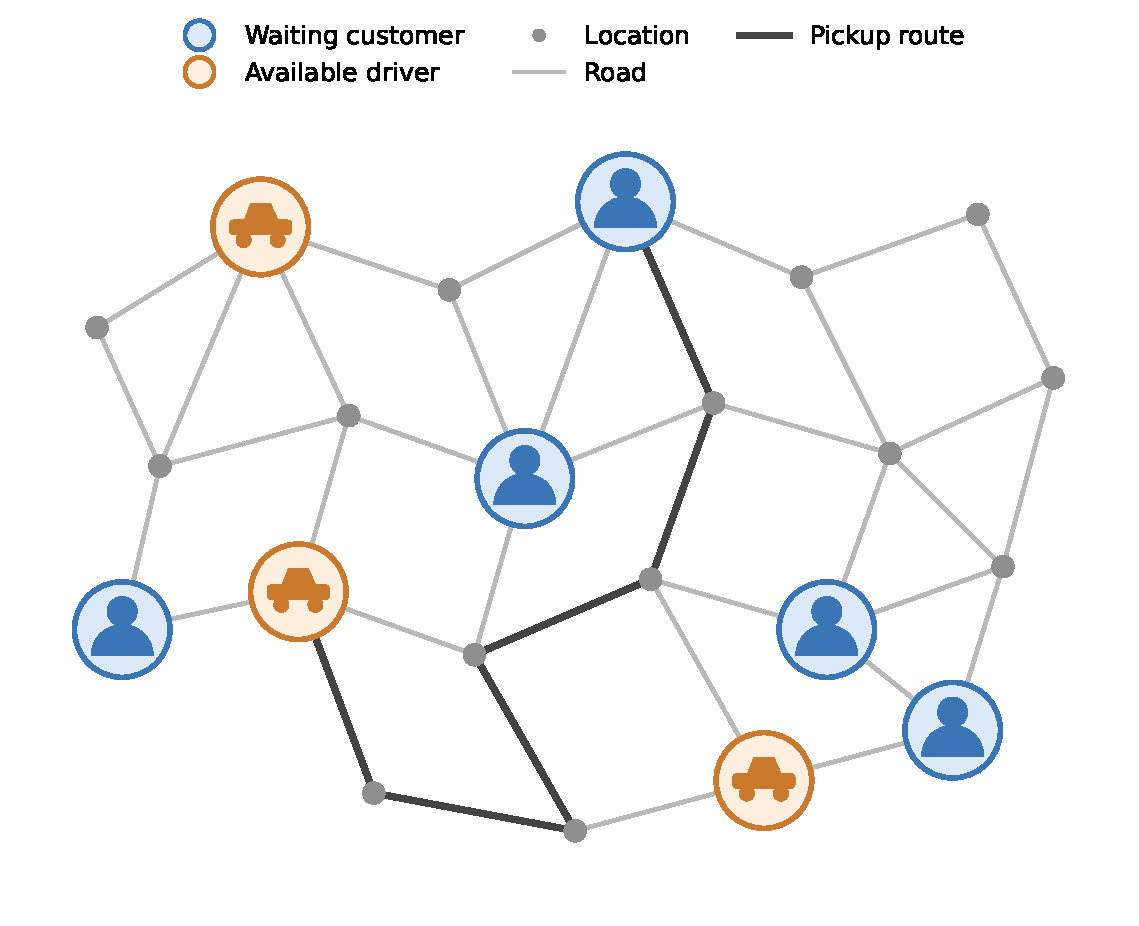
\includegraphics[width=\textwidth]{figures/ridesharing_illustration.pdf}
  \caption{Illustration of the ride-sharing problem}
  \label{fig:ride-sharing-illustration}
\end{figure}

Figure~\ref{fig:ride-sharing-illustration} illustrates the setting in a simple scenario. Customers wait at their pickup locations for a driver to be selected, and drivers wait for rides to be assigned. In reality, hundreds of customers may be waiting at a given moment, along with tens of drivers. Also, the number of locations is much larger in reality.

Simply put, this thesis studies the following problem: each customer provides their desired pickup time, destination location, and a list of drivers they are willing to be assigned to. Each driver has a shift with a fixed start and end time. A solution assigns customers to drivers and then determines the best schedule for each driver. In our problem, not all customers will be served. We measure the solution's performance by how many customers were not served, how long customers waited for pickup after their desired pickup times, and how much of the shift drivers spent idle.

\subsection{Motivation}

Despite having all the technology needed for successful ride-sharing, it has not grown as much as we expected~\citep{chan2012ridesharing}. The share of American workers commuting by carpool fell from 20.4 percent in 1970 to 10.7 percent in 2008~\citep{chan2012ridesharing}. Ride-sharing still accounts for only around 8 percent of trips in Canada and 11 percent in the United States, despite over 600 ride-matching programs operating there~\citep{chan2012ridesharing}. The problem is no longer connecting people, but deciding whom to connect with whom.

First, an algorithm that solves the ride-sharing problem quickly becomes complex, and using it can be time-consuming and possibly expensive. A system that matches thousands of customers to hundreds of drivers must solve a combinatorial optimisation problem constrained by the needs and wants of both groups~\citep{agatz2012optimization}. Also, because a matching system must respond within minutes, possibly seconds, it cannot compute an exact solution, as the classical dynamic programming solution to the single-vehicle dial-a-ride problem already requires computational effort that is exponential in the size of the problem~\citep{psaraftis1980dynamic,agatz2012optimization}. A natural solution is to split the problem into multiple smaller problems that are easier to solve independently, and to accept that the solution might no longer be completely optimal~\citep{agatz2012optimization}. This is a reasonable trade-off, and in this thesis we try an alternative approach to the problem.

Secondly, a solution is only useful if both the customers and drivers accept it. Trust, along with convenience and incentives, determines whether a person participates in a ride-sharing service at all~\citep{chaube2010trust}. Nevertheless, users are usually assumed to perform the screening rather than having it built into the matching~\citep{furuhata2013ridesharing}. Drivers are treated no better, as the objectives used in the literature are mostly system-wide or customer-facing, such as total vehicle-miles, total travel time, or the number of customers served~\citep{furuhata2013ridesharing,agatz2012optimization}. The driver appears mainly as a cost. A model that ignores either the customers or drivers can produce schedules that are optimal in theory but are refused in real-world use.

\subsection{Structure}

The rest of this thesis is organised as follows. Section~\ref{sec:literature-review} reviews the earlier work on ride-sharing and matching problems. Section~\ref{sec:methods} presents the thesis methodology. It introduces the problem statement, the three-step pipeline, the maximum-flow formulation of the matching problem, the integer linear program that schedules every driver, and the conflict-resolution step that ensures each customer is assigned to only one driver. Section~\ref{sec:experimental-settings} describes the synthetic test instances, the parameter values used in all instances, and the final results of each step. Section~\ref{sec:conclusion} summarises the findings, discusses the pipeline and formulation limitations, and outlines possible directions for future research.

\section{Literature Review}
\label{sec:literature-review}

Researchers have studied ways to solve the ride-sharing problem, as well as matching and scheduling, extensively over the last 20 years. The past literature approaches the ride-sharing problem from both operations research and systems perspectives. This section reviews the history of the ride-sharing problem, how it has been formulated and solved, and the history of matching and scheduling in the literature. 

The operations research view defines the problem as a routing problem and places it in the category of pickup-and-delivery problems, in which vehicles transport loads from origins to destinations~\citep{savelsbergh1995general}. The dial-a-ride problem is the special case where the loads are people~\citep{savelsbergh1995general}, ride-sharing is similar to the dynamic variant of the pickup-and-delivery problem~\citep{furuhata2013ridesharing}, and the customer experience is included in the objective~\citep{cordeau2007dialaride}. \citet{psaraftis1980dynamic} gives an exact dynamic programming algorithm for a single-vehicle many-to-many problem that minimizes a weighted combination of total service time and customer dissatisfaction. \citet{psaraftis1980dynamic} also shows that computational effort grows exponentially with problem size. Exact algorithms remain limited to small instances, while heuristics are the only methods that reach large ones~\citep{cordeau2007dialaride}. Also, in the dynamic case, where requests are revealed over time, a solution can no longer be a fixed plan but a strategy that reacts to new information~\citep{berbeglia2010dynamic}. The matching part of the problem has an even longer history as an assignment problem~\citep{pentico2007assignment}. Quite recently, \citet{masoud2017realtime} match each customer one at a time against all drivers, allowing riders to transfer between vehicles, and solve this many-to-one problem optimally with a dynamic program over a time-expanded network.

The literature that views the problem from a systems perspective investigates and builds matching programs to solve it. \citet{hall1997dynamic} studied dynamic ride-sharing, both analytically and through an implementation in Los Angeles, and found that a busy road produces a large enough pool of potential matches in theory. In practice, however, a customer had, at best, a one-in-five chance of being offered a ride per person contacted, even in an emergency. Hence, a match that is feasible in theory is not necessarily a match people accept~\citep{hall1997dynamic}. \citet{dailey1999seattle} moved matching to a series of web page forms, ran the system alongside a traditional phone-based program for a year, and reached about the same number of new users, suggesting that the matching mechanism does not limit it. Their model makes the number of matches proportional to the probability that two trips are compatible, so any restriction on a match lowers the number of matches formed~\citep{dailey1999seattle}. \citet{agatz2012optimization} survey the optimization side of the dynamic problem and conclude that centralized matching may be computationally infeasible for large cities, so a decomposition approach is necessary.

\subsection{Ride-sharing}

The term "ride-sharing" is not defined consistently in the literature. The broadest definition, by \citet{furuhata2013ridesharing}, defines it as a joint trip in which more than one participant shares a vehicle. \citet{furuhata2013ridesharing} also require participants to coordinate where and when each person is picked up and dropped off. \citet{chan2012ridesharing} add that the driver shares the same origin or destination as the passengers and does not financially benefit from the arrangement. \citet{agatz2012optimization} give a similar definition but also require that drivers are "independent private entities" and that trips are "single, non-recurring". \citet{mitropoulos2021systematic} find that, in the literature, the term is used for "both profit and non-profit ride-sharing services". \citet{pigalle2023ridesharing} separate ride-sharing from ride-hailing, which refers to the for-profit connection between riders and drivers. The organized variants share prearrangement by a service provider, which separates ride-sharing from hailing a taxi on the street~\citep{furuhata2013ridesharing}.

The literature is also divided by who runs the ride-sharing service. \citet{chan2012ridesharing} classify ride-sharing by the relationships among participants, separating acquaintance-based arrangements from organization-based ones where participants have a membership or join through a website. \citet{furuhata2013ridesharing} make a similar distinction on the provider side, distinguishing matching agencies that only introduce independent drivers and customers and service operators that have their own vehicles and drivers. These two cases have different problems. For an agency, both sides must screen the other side themselves, making trust a precondition for matching~\citep{chaube2010trust}. For an operator, they make most decisions, while the customer only needs to decide whether to take part~\citep{furuhata2013ridesharing}. This gives the fixed-fleet problem familiar from operations research, where vehicles have capacities and fixed start and end locations \comments{I coulnd't understand this sentence.}~\citep{savelsbergh1995general}, and requests can be turned down when the drivers cannot serve them~\citep{cordeau2007dialaride}. The scenario studied in this thesis falls into the operator category, where drivers work fixed shifts.

\subsection{Matching}

Matching customers to drivers is, in its most general form, an assignment problem, another category of problems which has a long history and many variants and algorithms~\citep{pentico2007assignment}. A classic assignment problem makes one-to-one assignments to minimize total cost, a problem that can be solved efficiently~\citep{pentico2007assignment, edmonds1972theoretical}. Ride-sharing differs in a few ways. The assignment is usually not a one-to-one matching, as a driver most likely serves several customers during a shift~\citep{savelsbergh1995general} and, when a matching agency does the matching, a customer is offered more than one driver to choose from~\citep{dailey1999seattle}. Also, the cost of an individual match is unknown before assignment because it depends on the driver's other matches. In the dial-a-ride problem, the feasibility of adding a request depends on the vehicle's current route~\citep{cordeau2007dialaride}. The objective can then be the number of matches rather than total cost, which \citet{agatz2012optimization} surveyed as an objective. Such a capacitated bipartite matching can be expressed as a maximum flow problem, in which the number of drivers a customer may be offered and the number of customers a driver may serve become edge capacities~\citep{ford1957simple}, and it is solvable in polynomial time with an integral solution~\citep{edmonds1972theoretical}.

\citet{masoud2017realtime} state that matching is integral to ride-sharing, and they incorporate time feasibility by matching a customer only when a feasible schedule exists for the ride. This avoids the poor scaling of exact dial-a-ride algorithms~\citep{cordeau2007dialaride}. The decision-maker in the matching also matters: when a service operator does the matching, it makes most decisions, whereas a matching agency introduces counterparts and leaves the decision to them \comments{Who's them here? It is a bit ambiguous}~\citep{furuhata2013ridesharing}. Under an operator, customer preferences can therefore enter the matching only as constraints. The preferences follow from the relationship between participants and the trust between the two sides~\citep{chaube2010trust}. Ride-sharing is sparse in time and space, which limits the number of customers that can be served~\citep{masoud2017realtime}, and the more preferences a customer has, the harder it is to find a suitable match~\citep{dailey1999seattle,agatz2012optimization}. This is consistent with the earlier observations that people do not always accept a match based on theory~\citep{hall1997dynamic}.

\subsection{Scheduling}

Choosing when each driver's ride takes place is a scheduling problem in the classical sense. In machine scheduling, each job has a processing time, a weight, a release date when the job becomes available, and a due date, and each machine can handle at most one job at a time~\citep{lenstra1977complexity}. In these terms, a driver is a single machine, a ride is a job whose processing time is the ride duration, and the wanted pickup time is the release date. The optimality criteria are functions of job completion times, such as maximum lateness, total tardiness, or the number of late jobs~\citep{lenstra1977complexity}. A late pickup is then a tardiness, and an unserved request equals a late job. \comments{Release dates alone make a single-machine problem hard. Not sure what this means.}. \citet{lenstra1977complexity} show that a non-zero release date for a single job is enough to make minimizing maximum lateness, total completion time, or the number of late jobs NP-complete \comments{It took a bit but I understood, but let us re-write this a bit}. Therefore, exact solutions rely on integer programming. \citet{dyer1990formulating} compare several formulations of the single-machine problem with release dates and conclude that formulations based on time discretization give the best lower bounds. In their best formulation, a binary variable equals one if a job starts processing at a given time, which makes the feasible set essentially independent of the data but gives the formulation a very large number of variables~\citep{dyer1990formulating}. However, classical criteria do not measure the machine, since they are all functions of job completion times~\citep{lenstra1977complexity} \comments{Might need an extra explanation}. In the dial-a-ride problem, the vehicle's waiting time at a stop is a scheduling variable, and some variants bound it from above, but drivers remain in the objective only through their wages~\citep{cordeau2007dialaride}.

In the dial-a-ride literature, the scheduling step follows the routing step~\citep{cordeau2007dialaride,savelsbergh1995general}. Given a route, the scheduling problem determines the departure time from the depot and the time the ride begins at each stop so that the time constraints are satisfied and the route duration is minimized~\citep{cordeau2007dialaride}. For a fixed route, this is altrivial, as the optimal departure time can be determined in time linear in the length of the route~\citep{cordeau2007dialaride}. The difficulty comes from choosing the route, since for a single vehicle the exact dynamic program of \citet{psaraftis1980dynamic} grows exponentially in the number of requests. Multi-vehicle methods therefore decompose the problem~\citep{savelsbergh1995general,cordeau2007dialaride} \comments{I think that something is missing here}. A common technique defines customer clusters to be served by the same driver before the routing phase, and then solves each cluster using a single-vehicle algorithm~\citep{cordeau2007dialaride,savelsbergh1995general}. Some other methods alternate between a routing step and a scheduling step~\citep{cordeau2007dialaride,savelsbergh1995general}. Once a driver's customers are assigned and each ride is defined as a block of time, we have the single-machine problem described above for each vehicle. The clusters are not independent, however, and early cluster-first \comments{Let us use a different word here} heuristics already switch between clusters after solving each one~\citep{cordeau2007dialaride}. \citet{agatz2012optimization} note that a geographic partition can be problematic because a ride's origin and destination may fall in different subregions. \citet{masoud2017realtime} take the opposite route and keep time feasibility inside the matching, constructing a time-expanded feasible network for one rider at a time and searching it with a dynamic program, at the cost of processing the riders one after another.

\subsection{Contribution}

This thesis investigates the problem by decomposing it into matching, per-driver scheduling, and conflict resolution, following the decomposition that \citet{agatz2012optimization} expect to be necessary. Matching on the preference graph alone is inexpensive, since maximum flow is solvable in polynomial time~\citep{edmonds1972theoretical}, and it reduces each driver's candidate set before scheduling. The conflict resolution step plays the role of the swaps between clusters that the cluster-first \comments{same here} heuristics make after solving each cluster~\citep{cordeau2007dialaride}.

We add customer preferences as hard constraints to the matching instead of relying on users to screen for their driver. The customers' preferences form a bipartite graph in which suitable drivers are matched to each customer. In practice, screening is done by manual selection from stored participant profiles~\citep{furuhata2013ridesharing}; whether a match is accepted depends on trust between the parties~\citep{chaube2010trust}; and restrictions are treated as something that makes matching harder~\citep{agatz2012optimization}. \citet{furuhata2013ridesharing} identify integrating screening into the ride-matching itself, which they call high-dimensional matching, as an open challenge, and note that screening items treated as hard constraints are the simple case. This thesis takes that simple case: each customer's list of acceptable drivers is a hard constraint on the matching.

Past literature also rarely accounts for drivers when forming model objectives, and it often uses decomposition. Drivers usually appear only as wage costs~\citep {cordeau2007dialaride}. Instead, we add driver idle time as a term in the objective and try to minimize it. Arguably, we should also account for driver experience, which we investigate here.
\section{Methods}
\label{sec:methods}

In this section, we describe the methodology we use to solve the ride-sharing problem. First, we state the problem, then briefly introduce the pipeline, followed by a detailed discussion of each step. As discussed before, a multi-driver ride-sharing problem is computationally difficult to solve in a reasonable runtime. Due to this, we introduce a decomposed, three-step approach rather than trying to formulate the problem as a single integer linear program.

\subsection{Problem formulation}

Let $\mathcal{N}$ be the set of customers and $\mathcal{K}$ the set of drivers. Each customer $i$ has a set $\mathcal{P}_i\subset\mathcal{K}$ of driver preferences. Customer $i$ can be assigned to driver $k$ only if $ k$ is in customer $ i$'s preference set. This relationship between customers and drivers can be modelled using a graph.

\begin{definition}[Graph]
A \emph{graph} $G = (V, E)$ consists of a finite set $V$ of \emph{vertices} and a set $E$ of \emph{edges}, where each edge $\{u, v\} \in E$ joins two distinct vertices $u, v \in V$. Each edge also carries a number $w(e)$, making the graph a \emph{weighted graph}.
\end{definition}

The sets $\mathcal{N}$ and $\mathcal{K}$ form two disjoint sets of vertices. These sets can be connected uniquely by connecting each vertex $i\in\mathcal{N}$ to all vertices in $\mathcal{P}_i$. Since $\mathcal{P_i}\subset\mathcal{K}$, a vertex $i\in\mathcal{N}$ can be connected only to a vertex $k\in\mathcal{K}$, making the graph bipartite. 

\begin{definition}[Bipartite graph]
A graph is \emph{bipartite} if its vertex set can be partitioned into two disjoint sets $V = A \cup B$ such that every edge joins a vertex in $A$ to a vertex in $B$.
\end{definition}

Each customer $i$ has a wanted pickup time $U_i$ and a ride duration $R_i$, and each driver $k$ works within a shift window $[S_k, H_k]$, meaning the driver is available from time $S_k$ until time $H_k$. 

The objective is to calculate optimal schedules for each driver to minimise the number of unserved customers, customer pickup delays, and driver idle time. This means finding a suitable set of customers for each driver. We define the problem as a combination of matching and optimisation. 

\begin{definition}[Matching]
A \emph{matching} in a graph is a set of edges of which no two share a vertex. We use a capacitated generalization in which each vertex $v$ may be connected by at most $c(v)$ chosen edges, where $c(v)$ is a per-vertex capacity.
\end{definition}

The idea is to first find, for each driver $k$, an assignable set $A_k \subseteq \mathcal{N}$ of customers by computing a matching on the preference graph. Then, using the assignable sets, we optimize an initial schedule for each driver with integer linear programming (ILP). Because drivers are scheduled independently, a single customer can be assigned to several drivers, causing conflicts. To resolve the conflicts, we perform a conflict-resolution step and iterate the scheduling to improve the total objective value. As a result, we have three separate problems to define and solve.

These three subproblems, matching, scheduling and conflict resolution, together form a pipeline that finds a solution to the whole scheduling problem. It takes the bipartite graph of preferences as input and produces optimised schedules and a set of metrics as output. Figure~\ref{fig:pipeline} shows the pipeline overview.

\begin{figure}[H]
  \centering
  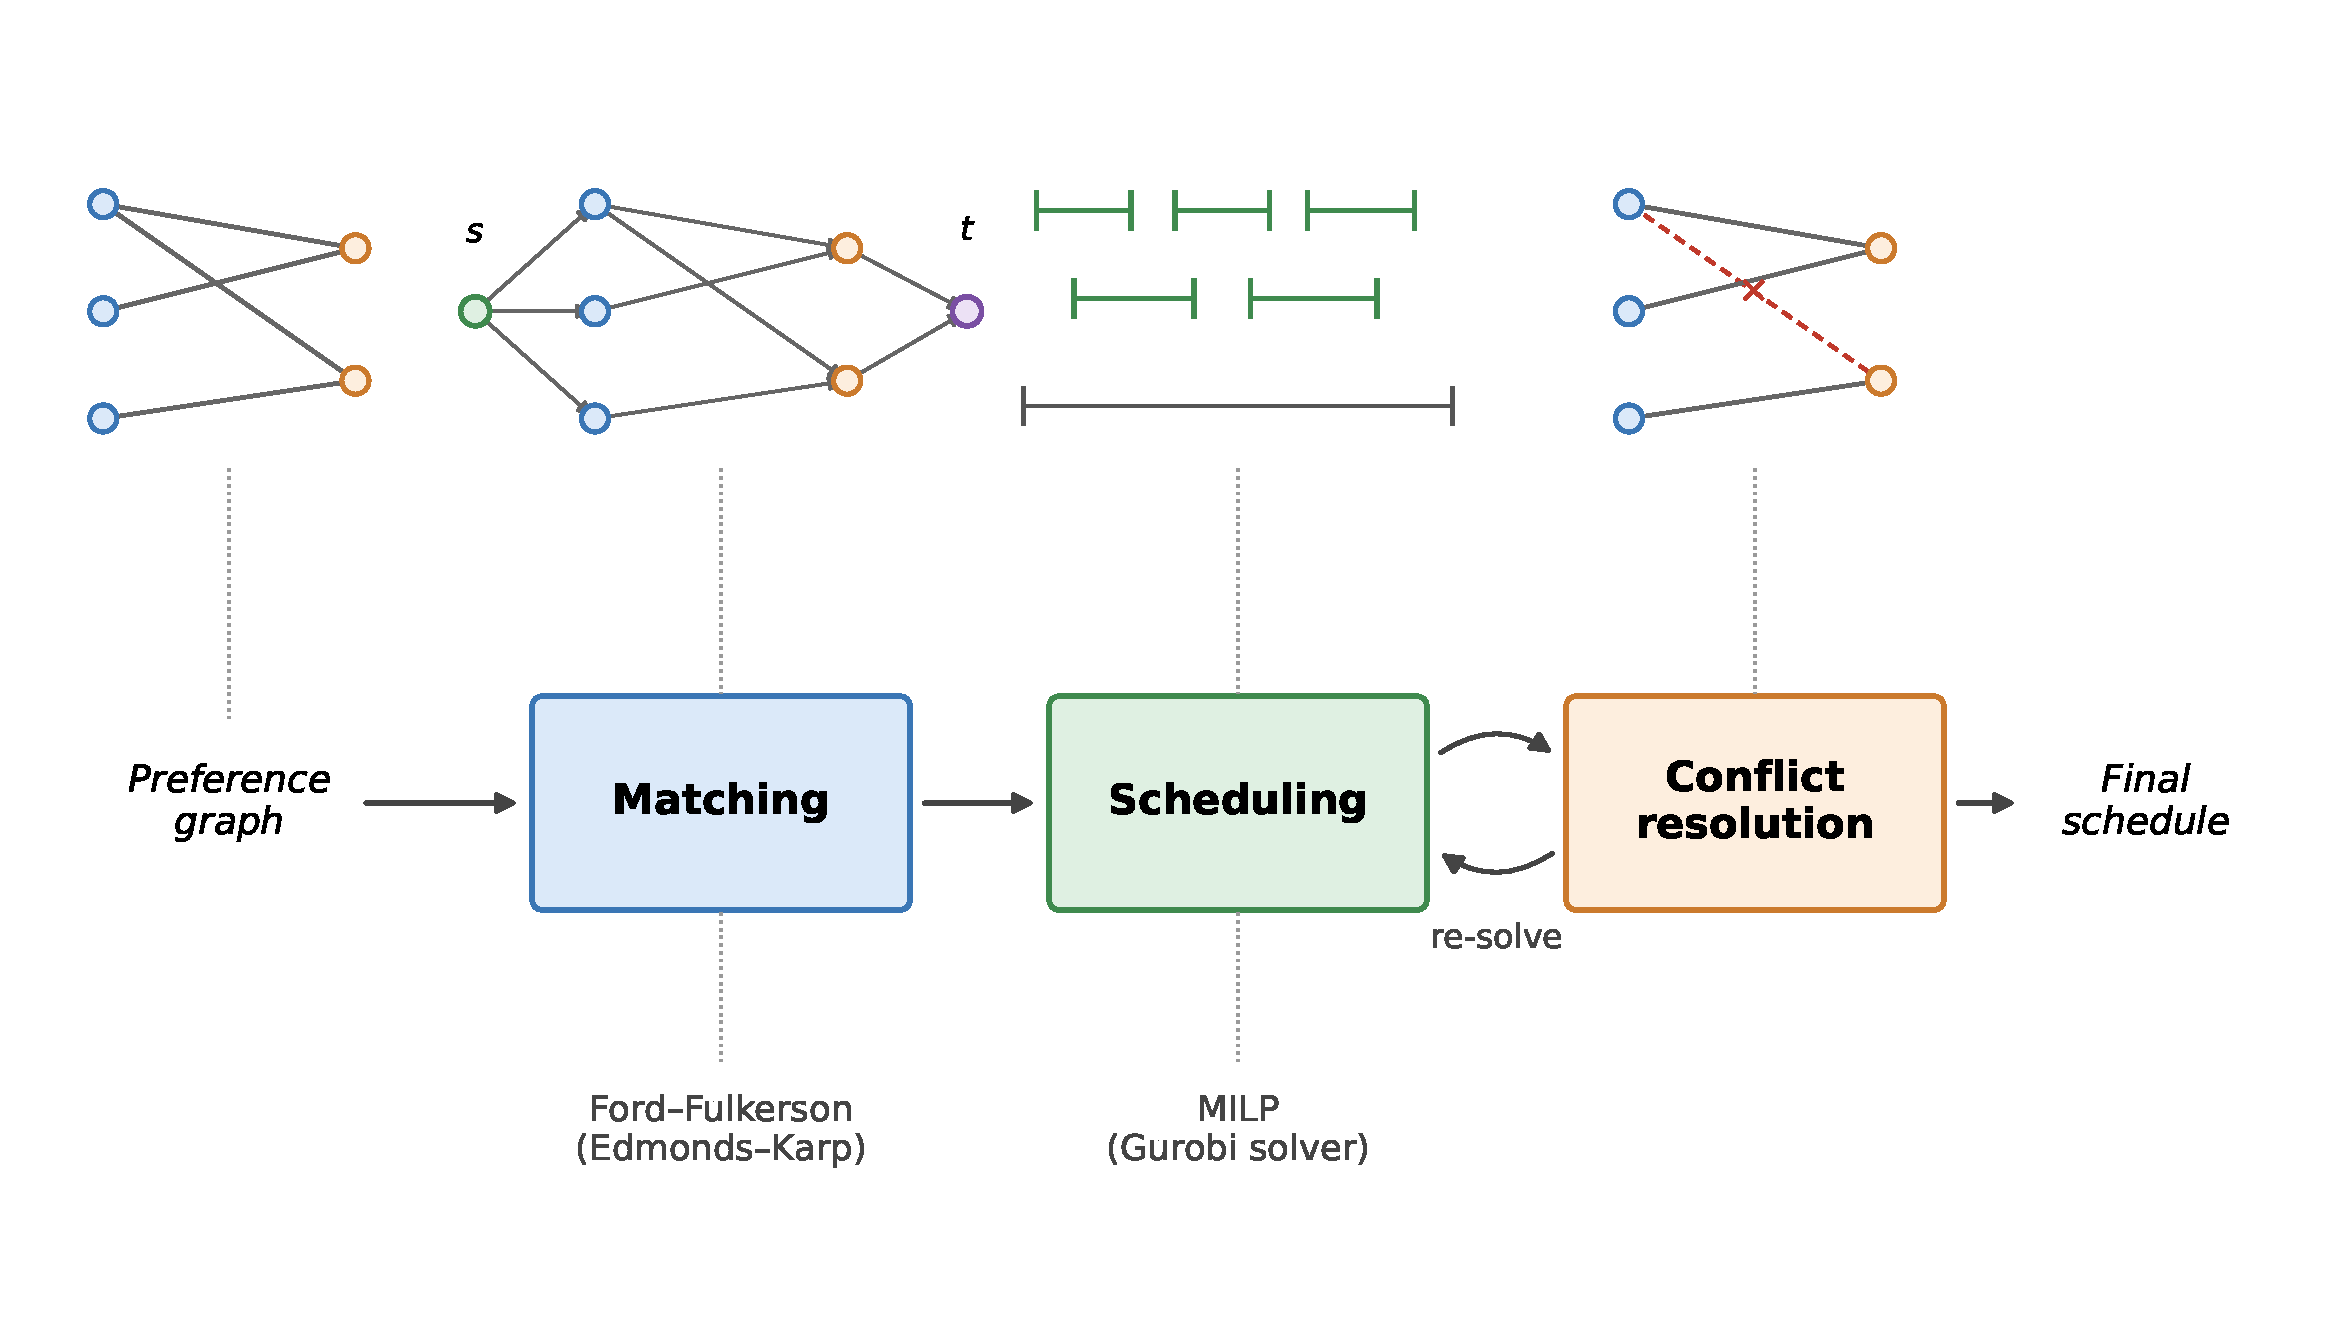
\includegraphics[width=1.05\textwidth]{figures/pipeline_process_flow.pdf}
  \caption{The outline of the scheduling pipeline}
  \label{fig:pipeline}
\end{figure}

\subsection{Matching via maximum flow}

The first subproblem in the scheduling pipeline is matching. Each customer $i$ provides a set of driver preferences $\mathcal{P}_i$, and the number of drivers a customer can be matched to is capped. A driver can be matched to as many customers as possible. The matching subproblem provides the assignable sets $A_k$ for each driver $k$ as output. We formulate the subproblem as a capacitated bipartite matching problem.

\begin{problem}[Matching customers to drivers]
\label{prob:matching}
Let $G = (\mathcal{N} \cup \mathcal{K}, E)$ be the bipartite preference graph with an edge set 
\[
E = \bigl\{\, \{i, k\} : i \in \mathcal{N},\ k \in \mathcal{P}_i \,\bigr\}
\]
and let $w(i) \in \mathbb{Z}$ be the weight of customer $i$, that is, the maximum number of drivers customer $i$ may be matched to and let $w(k) \in \mathbb{Z}$ be the weight of driver $k$, that is, the maximum number of customers driver $k$ may serve.\\
Find a matching $M \subseteq E$ of maximum cardinality that respects the weights, i.e. solve
\begin{align}
  \max_{M \subseteq E} \quad & |M| \label{eq:matching-obj}\\
  \text{s.t.} \quad
  & \bigl|\{\, k : \{i,k\} \in M \,\}\bigr| \le c(i) && \text{for all } i \in \mathcal{N}, \label{eq:matching-cust}\\
  & \bigl|\{\, i : \{i,k\} \in M \,\}\bigr| \le c(k) && \text{for all } k \in \mathcal{K}. \label{eq:matching-drv}
\end{align}
The matching $M$ defines an assignable set for each driver $k$
\[
A_k = \bigl\{\, i \in \mathcal{N} : \{i, k\} \in M \,\bigr\}.
\]
\end{problem}

We solve Problem~\ref{prob:matching} using maximum flow with the Ford––Fulkerson algorithm~\citep{ford1957simple}. The Ford–Fulkerson algorithm computes the maximum flow in a directed graph. Ford–Fulkerson constructs a copy of the original graph, called the residual graph, and uses it to compute the maximum flow by repeatedly finding augmenting paths. An augmenting path is a path through the graph with remaining capacity. We use a variant of the Ford–Fulkerson algorithm called the Edmonds–Karp algorithm~\citep{edmonds1972theoretical}, which computes augmenting paths using breadth-first search. Algorithm~\ref{alg:ff} provides the algorithm pseudocode. We record the wall-clock time for the matching process so we can report the Ford–Fulkerson runtime alongside the solution.

\begin{algorithm}[H]
\caption{Ford–Fulkerson with breadth-first search (Edmonds–Karp)}
\label{alg:ff}
\begin{algorithmic}[1]
\Require directed graph $G = (V, E)$ with capacities $w$, source $s$, sink $t$
\Ensure the maximum flow value $f$
\ForAll{$(u, v) \in E$} \Comment{initialize the residual capacities}
  \State $r(u, v) \gets w(u, v)$
  \State $r(v, u) \gets 0$
\EndFor
\State $f \gets 0$
\Loop
  \State find a shortest path $p$ from $s$ to $t$ using breadth-first search over the edges with $r(u, v) > 0$
  \If{no such path exists}
    \State \Return $f$
  \EndIf
  \State $b \gets \min_{(u, v) \in p} r(u, v)$ \Comment{bottleneck of the path}
  \ForAll{$(u, v) \in p$} \Comment{push $b$ units of flow along $p$}
    \State $r(u, v) \gets r(u, v) - b$
    \State $r(v, u) \gets r(v, u) + b$
  \EndFor
  \State $f \gets f + b$
\EndLoop
\end{algorithmic}
\end{algorithm}

To compute the maximum flow, the Ford–Fulkerson algorithm needs a single source, a vertex where all flow is created, and a single sink, a vertex where all flow is consumed. We add these vertices so the source connects to every customer vertex and the sink to every driver vertex. The weights of the outgoing edges from a source set how many drivers a customer may choose from, and the weights of the incoming edges to a sink set a driver's capacity. Figure~\ref{fig:bipartite} shows the resulting
bipartite structure with the added source and sink.

\begin{figure}[H]
  \centering
  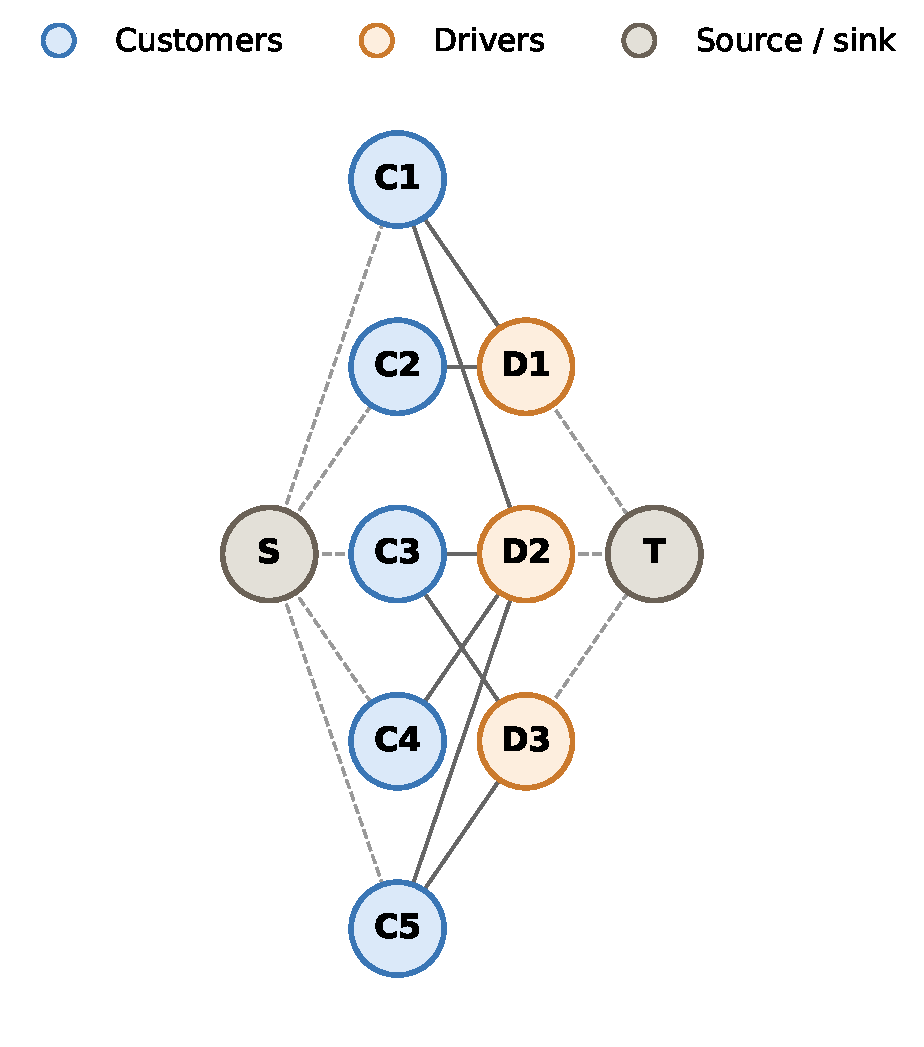
\includegraphics[height=0.6\textheight]{figures/bipartite_graph.pdf}
  \caption{A bipartite customer-driver graph with the source and sink.}
  \label{fig:bipartite}
\end{figure}

The customer-driver matching is read from the residual graph. For every edge $(c, d)$ between a customer $c$ and a driver $d$ in the original graph, the flow used along that edge equals the original capacity minus the remaining residual capacity. If this used flow is strictly positive, we record $(c, d)$ as a matched pair. From these matched pairs, we construct the sets of assignable customers. We record the average number of customers per driver, drivers per customer and also the coverage percentage, that is, the share of customers that were matched to at least one driver.

\subsection{Per-driver scheduling ILP}

After the matching step, we solve each driver's schedule separately using integer linear programming. The matching subproblem provides, for each driver $k$, the set $A_k$ of customers that $k$ is allowed to serve. This subproblem provides the initial schedules of each driver $k$ as output. A customer may be assigned to multiple drivers as the drivers are scheduled independently.

\begin{problem}[Scheduling customers for a driver]
\label{prob:scheduling}
Let $k$ be a driver with a shift window $[S_k, H_k]$ and an assignable set $A_k$ and let each customer $i \in A_k$ have a wanted pickup time $U_i$ and a ride duration $R_i$. Find a set $C_k \subseteq A_k$ of served customers and a pickup time $t_i$ for each $i \in C_k$ such that
\begin{enumerate}
  \item each ride lies within the shift and its pickup delay is bounded: $\max(U_i, S_k) \le t_i \le U_i + E_{\max}$ and $t_i + R_i \le H_k$,
  \item the rides of driver $k$ do not overlap, and the break between two consecutive rides is at least $B_{\min}$ and at most $B_{\max}$ minutes,
  \item the last ride ends within $B_{\max}$ minutes of the shift end $H_k$,
\end{enumerate}
minimizing the weighted sum
\[
D \sum_{i \in C_k} (t_i - U_i)
+ P\,\bigl|A_k \setminus C_k\bigr|
+ I \Bigl( (H_k - S_k) - \sum_{i \in C_k} R_i \Bigr)
\]
of the total pickup delay, the number of unserved customers, and the driver's idle time, with given weights $D$, $P$, and $I$.
\end{problem}

We solve Problem~\ref{prob:scheduling} with an independent time-indexed ILP for each driver $k$. We discretise time into slots of width $\Delta t$, one minute by default. For every customer $i \in A_k$ and every feasible start slot $t$, we introduce a binary variable $x_{i,t} \in \{0, 1\}$ that equals one if and only if customer $i$'s ride starts at slot $t$ on driver $k$. A start slot $t$ is feasible if and only if

\begin{align}
t \cdot \Delta t        &\geq \max(U_i, S_k), \label{eq:feas-start} \\
t \cdot \Delta t + R_i  &\leq H_k, \label{eq:feas-end} \\
t \cdot \Delta t - U_i  &\leq E_{\max}. \label{eq:feas-delay}
\end{align}

Constraint~\eqref{eq:feas-start} schedules the customer's pickup after both their wanted pickup time and the driver's shift start, \eqref{eq:feas-end} ensures the ride ends before the end of the driver's shift, and \eqref{eq:feas-delay} caps the pickup delay at $E_{\max}$. Let $T_i$ denote the set of feasible start slots for customer $i$ on driver $k$ and let $e_{i,t} = t \cdot \Delta t + R_i$ be the end of ride $(i,t)$. Let $N_{i,t} = \{(j, t') : j \in A_k \setminus \{i\},\ t' \in T_j, e_{i,t} < t' \cdot \Delta t \leq e_{i,t} + B_{\max}\}$ be the rides that could follow $(i,t)$, that is, those starting within $B_{\max}$ minutes of its end. Let $r_i = \lceil R_i / \Delta t \rceil$ be the number of slots a ride covers. To enforce a minimum break of $B_{\min}$ minutes between consecutive rides, inflate each ride's time footprint from $r_i$ to $r_i + b$, where $b = \lceil B_{\min} / \Delta t \rceil$. The ILP is

\begin{align}
\min \quad & D \sum_{i \in A_k} \sum_{t \in T_i} (t \cdot \Delta t - U_i) x_{i,t} \\
    +\quad & P \sum_{i \in A_k} ( 1 - \sum_{t \in T_i} x_{i,t} ) \\
    +\quad & I ( (H_k - S_k) - \sum_{i \in A_k} \sum_{t \in T_i} R_i x_{i,t} ) \label{eq:obj} \\
\text{s.t.} \quad 
\sum_{t \in T_i} x_{i,t} &\leq 1, && \forall i \in A_k, \label{eq:assign} \\
\sum_{\substack{i \in A_k, \, t \in T_i \\ t \leq \tau < t + r_i + b}} x_{i,t} &\leq 1, && \forall \text{ slot } \tau, \label{eq:overlap} \\
x_{i,t} &\leq \sum_{(j,t') \in N_{i,t}} x_{j,t'}, && \forall (i,t) \text{ s.t. } e_{i,t} + B_{\max} < H_k, \label{eq:succ} \\
& x_{i,t} \in \{0, 1\}, && \forall i \in A_k, \, t \in T_i. \label{eq:integrality}
\end{align}

The objective~\eqref{eq:obj} has three terms. The first minimizes total pickup delay, weighted by $D$. The second penalises each unserved customer by $P$. The third term, weighted by $I$, penalises the driver's idle time over the shift. Constraint~\eqref{eq:assign} serves each customer at most once, and \eqref{eq:overlap} forbids overlapping rides on the same driver by allowing at most one active ride in any slot $\tau$. Constraint~\eqref{eq:succ} bounds the breaks between rides to a maximum of $B_{\max}$ by requiring each ride to have a successor during the subsequent $B_{\max}$ minutes if there are more than $B_{\max}$ minutes of the driver's shift left after the drop-off of that ride. 

We use Gurobi (\citep{gurobi}) to optimize the ILPs. As the ILPs are independent of each other, we utilize parallelization to solve them in a less amount of time. From the solution, for each assigned customer $i$, we read their chosen start slot and realised pickup delay $\max(0,\, t \cdot \Delta t - U_i)$.

\subsection{Conflict resolution between drivers}

Since we scheduled each driver independently in the scheduling subproblem, the same customer can be assigned to more than one driver. Thus, we need to resolve conflicts between drivers so that each customer is served by at most one driver.

\begin{problem}[Conflict resolution]
\label{prob:conflict}
For each driver $k \in \mathcal{K}$, let $(C_k, (t_i)_{i \in C_k})$ be the solution of Problem~\ref{prob:scheduling}. A customer $i$ is \emph{contested} if $i \in C_k \cap C_l$ for two distinct drivers $k \ne l$. Find pairwise disjoint served sets $C'_k \subseteq A_k$ and pickup times $t'_i$ for each $i \in C'_k$ such that every $(C'_k, (t'_i)_{i \in C'_k})$ satisfies the constraints of Problem~\ref{prob:scheduling}, minimizing
\[
D \sum_{k \in \mathcal{K}} \sum_{i \in C'_k} (t'_i - U_i)
+ P \Bigl( |\mathcal{N}| - \sum_{k \in \mathcal{K}} |C'_k| \Bigr)
+ I \sum_{k \in \mathcal{K}} \Bigl( (H_k - S_k) - \sum_{i \in C'_k} R_i \Bigr),
\]
the total objective of Problem~\ref{prob:scheduling} summed over all drivers, with each customer now counted as served if any driver serves them.
\end{problem}

We solve Problem~\ref{prob:conflict} using a greedy resolution loop. For each customer assigned to at least two drivers, assign them to the driver with the lowest pickup delay. We then remove the customer from the assignable sets and schedules of all other drivers. This resolves all conflicts but is only the first part of the solution to the subproblem.

After removing the contested customers from drivers' assignable sets, previously unserved customers may now be assignable. Because of this, we iteratively resolve the per-driver scheduling problems. In each round, we rerun every driver's ILP on the union of its current assignments and the customers that are still unserved but lie in the driver's assignable set. Any customer a resolved ILP newly assigns is removed from the unserved pool immediately. We stop when a round changes no driver's assignments, when the unserved customer pool fails to shrink between rounds or after a configurable round limit, whichever comes first.

Because the order in which drivers are processed affects the outcome of the greedy conflict resolution loop, we run conflict resolution with five different driver orderings and keep the best result. The five comparators are ascending index, ascending number of customers, descending number of customers, ascending number of conflicts and descending number of conflicts. Also, since the loop is greedy, we only compute the different orderings in parallel and not all of the ILPs like in the scheduling subproblem. Algorithm~\ref{alg:conflict} summarises the full procedure.

\begin{algorithm}[H]
\caption{Conflict resolution between drivers}
\label{alg:conflict}
\begin{algorithmic}[1]
\Require per-driver schedules from the first ILP pass, assignable sets $A_k$
\Ensure an assignment of each customer to at most one driver
\ForAll{customers $i$ chosen by at least one driver} \Comment{greedy resolution}
  \State assign $i$ to the choosing driver with the lowest pickup delay for $i$, breaking ties by the lowest driver index
\EndFor
\ForAll{driver orderings $\sigma$ of the five comparators}
  \State start from the greedy assignment; $Q \gets$ unserved customers
  \For{$\mathrm{round} = 1, \dots, \mathrm{round\ limit}$} \Comment{iterated conflict resolution}
    \ForAll{drivers $k$ in the order $\sigma$}
      \State $C_k \gets \{\text{customers currently assigned to } k\} \cup (Q \cap A_k)$
      \If{$C_k$ differs from $k$'s previous input}
        \State resolve driver $k$'s ILP over $C_k$
        \State assign each customer served by the new schedule to $k$ and remove them from $Q$
        \State return each customer no longer served by $k$ to $Q$
      \EndIf
    \EndFor
    \If{no driver's schedule changed during the round}
      \State \textbf{break}
    \EndIf
    \If{$\mathrm{round} > 1$ and $Q$ did not shrink during the round}
      \State \textbf{break}
    \EndIf
  \EndFor
\EndFor
\State \Return the assignment of the ordering with the lowest objective value
\end{algorithmic}
\end{algorithm}
\section{Experimental Settings}
\label{sec:experimental-settings}

In this section, we go through the experiments performed on our pipeline. We describe the parameter values and data used in the testing of each subproblem. Then, we present the results and briefly discuss them.

The implementation and the code used to generate each tested scenario are public and available in the following \href{https://github.com/aapolaakkio/thesis}{GitHub repository}.

\subsection{Data}

The data used to test the pipeline is synthetic, meaning it is randomly generated. We sample a per-graph scenario using a fixed graph id as the random-number-generator seed to ensure reproducibility. Each driver $k$ is assigned a shift start time $S_k\sim U(0, 60)$ and shift end time $H_k\sim U(240, 600)$, which together form the driver's shift window $[S_k, H_k]$, with both ends drawn from a uniform distribution. Each customer $i$ is drawn a wanted pickup time $U_i\sim U(0, 600)$ and a ride duration $R_i\sim U(5, 30)$. A delay cap $E_{\max}=15$ bounds how late a pickup can occur relative to the customer's wanted pickup time. Minimum break length $B_{\min}=10$ and maximum break length $B_{\max}=60$ are used to ensure some time between rides, simulating needing to move to a different location for the next pickup. We set the customer pickup delay and driver idle-time multipliers to $D=1$ and $I=1$. We charge a penalty $P=300$ for every customer that ends up unassigned.

We configure the bipartite graphs to have 3-6 edges for each customer, meaning 3-6 preferences per customer. We also allow at most 5 matched drivers for each customer. For drivers, we do not cap the number of matched customers, so theoretically all customers can be assigned to a single driver. In addition, we set the time granularity $\Delta t=1$, meaning scheduling is done at one-minute precision; we limit the resolution to at most 5 rounds, and each Gurobi run to at most 30 seconds.

We run 18 scenarios and one reference scenario. The number of customers was set as $N\in\{6000,7000,8000\}$ and number of drivers as $K\in\{100,110,120,130,140,150\}$. We run a scenario for every customer and driver count pair $N \times K$. We also run one additional reference with $N=1000$ and $K=200$ to test the pipeline's sensitivity.

\subsection{Matching results}

The first subproblem is finding the matching via maximum flow computation. For this subproblem, we record the maximum flow computed by the Ford–Fulkerson algorithm (max-flow), the time to compute the maximum flow and the matching ($t_{\text{FF}}$), the average customers per driver (cust./drv.) and average drivers per customer (drv./cust.). The results are presented in Table~\ref{tab:matching}.

\begin{table}[H]
\centering
\caption{Matching results}
\label{tab:matching}
\begin{tabular}{rrrrrr}
\toprule
$N$ & $K$ & max-flow & $t_{\text{FF}}$ (s) & cust./drv. & drv./cust. \\
\midrule
1000 & 200 & 4280 & 1.8  & 21.4 & 4.28 \\
6000 & 100 & 25469 & 65.4  & 254.7 & 4.24 \\
6000 & 110 & 25470 & 62.6  & 231.5 & 4.25 \\
6000 & 120 & 25511 & 62.4  & 212.6 & 4.25 \\
6000 & 130 & 25581 & 63.9  & 196.8 & 4.26 \\
6000 & 140 & 25516 & 64.9  & 182.3 & 4.25 \\
6000 & 150 & 25627 & 64.3  & 170.8 & 4.27 \\
7000 & 100 & 29805 & 85.7  & 298.1 & 4.26 \\
7000 & 110 & 29887 & 87.6  & 271.7 & 4.27 \\
7000 & 120 & 29644 & 85.6  & 247.0 & 4.23 \\
7000 & 130 & 29884 & 89.1  & 229.9 & 4.27 \\
7000 & 140 & 29759 & 87.1  & 212.6 & 4.25 \\
7000 & 150 & 29734 & 87.5  & 198.2 & 4.25 \\
8000 & 100 & 33933 & 113.3  & 339.3 & 4.24 \\
8000 & 110 & 34079 & 120.0  & 309.8 & 4.26 \\
8000 & 120 & 33963 & 113.4  & 283.0 & 4.25 \\
8000 & 130 & 34025 & 115.1  & 261.7 & 4.25 \\
8000 & 140 & 34011 & 121.0  & 242.9 & 4.25 \\
8000 & 150 & 34056 & 120.4  & 227.0 & 4.26 \\
\bottomrule
\end{tabular}
\end{table}

We observe that the maximum flow steadily increases as both the number of customers and the number of drivers increases. Increments in the number of customers cause a larger increase in the maximum flow than increments in the number of drivers. We also observe that the time to calculate the matching grows superlinearly with the number of customers, from an average of 64 seconds at $N = 6000$ to 117 seconds at $N = 8000$, and decreases slightly with the number of drivers.

The averages, however, behave a little differently. The average customers per driver increases as the number of customers increases but decreases as the number of drivers increases. This is logical, as drivers can match to a customer as long as there is an edge between them. Since drivers have no limit to the number of matched customers, only the number of edges generated between vertices limits the average. 

On the other hand, drivers per customer is almost the same across scenarios, averaging around $4.25$. This naturally happens because of the cap of 5 drivers per customer, and since there are always 3-6 edges per customer vertex, customers are matched to an average of $\frac{3+4+5+5}{4}=4.25$ drivers.

\subsection{Scheduling results}

The second subproblem is the per-driver scheduling. From this subproblem, we record the structure of the delivered schedule, i.e. the number of assigned (assig.) and unassigned customers (unassig.), the number of drivers that serve at least one customer (drv.\ used), the maximum (max load) and average number of customers per driver (avg load), the total pickup delay (delay) and idle time in minutes (idle), and the runtime of the first scheduling pass in seconds  ($t_{\text{sched}}$). Table~\ref{tab:scheduling} presents the results, and Figure~\ref{fig:sched-runtime} plots the runtime.

\begin{table}[H]
\centering
\caption{Scheduling results}
\label{tab:scheduling}
\small
\begin{tabular}{rrrrrrrrrr}
\toprule
$N$ & $K$ & assig. & unassig. & drv.\ used & max load & avg load & delay & idle & $t_{\text{sched}}$ \\
\midrule
1000 & 200 & 674 & 326 & 166 & 13 & 4.1 & 1642 & 64099 & 1.3 \\
6000 & 100 & 1789 & 4211 & 100 & 29 & 17.9 & 6914 & 18556 & 7.5 \\
6000 & 110 & 1818 & 4182 & 110 & 29 & 16.5 & 7039 & 19036 & 5.3 \\
6000 & 120 & 2069 & 3931 & 120 & 27 & 17.2 & 8408 & 21742 & 5.6 \\
6000 & 130 & 2202 & 3798 & 130 & 29 & 16.9 & 8430 & 23199 & 5.8 \\
6000 & 140 & 2290 & 3710 & 140 & 26 & 16.4 & 8801 & 24204 & 5.4 \\
6000 & 150 & 2442 & 3558 & 150 & 28 & 16.3 & 9159 & 26167 & 4.8 \\
7000 & 100 & 1835 & 5165 & 100 & 28 & 18.4 & 6960 & 19039 & 8.6 \\
7000 & 110 & 1935 & 5065 & 110 & 27 & 17.6 & 7803 & 20008 & 7.3 \\
7000 & 120 & 2165 & 4835 & 120 & 28 & 18.0 & 8568 & 22510 & 7.3 \\
7000 & 130 & 2371 & 4629 & 130 & 27 & 18.2 & 8759 & 24870 & 7.6 \\
7000 & 140 & 2524 & 4476 & 140 & 28 & 18.0 & 9180 & 26661 & 7.8 \\
7000 & 150 & 2675 & 4325 & 150 & 27 & 17.8 & 9804 & 28126 & 6.8 \\
8000 & 100 & 1877 & 6123 & 100 & 30 & 18.8 & 7597 & 19358 & 11.1 \\
8000 & 110 & 2087 & 5913 & 110 & 29 & 19.0 & 7872 & 21636 & 10.1 \\
8000 & 120 & 2219 & 5781 & 120 & 29 & 18.5 & 8276 & 23051 & 9.1 \\
8000 & 130 & 2380 & 5620 & 130 & 29 & 18.3 & 9181 & 24851 & 10.4 \\
8000 & 140 & 2490 & 5510 & 140 & 28 & 17.8 & 9562 & 26030 & 10.7 \\
8000 & 150 & 2758 & 5242 & 150 & 28 & 18.4 & 10865 & 28932 & 10.7 \\
\bottomrule
\end{tabular}
\end{table}

In every scenario, the number of served customers is limited by the driver capacity, not by the matching done in the previous subproblem. A driver's shift is on average about 390 minutes long, and a served ride takes on average $17.5 + B_{\min} = 27.5$ minutes, so a driver can serve roughly 14--26 customers depending on ride lengths. The observed maximum loads of 26--30 sit at the top of this range. Consequently, the number of assigned customers grows almost linearly with the number of drivers, by roughly 13 customers per added driver, while thousands of customers remain unassigned. Increasing the number of customers at a fixed driver count increases the assigned count only slightly. More customers give each driver more short rides to choose from, allowing denser packing of their shifts. Because every unassigned customer costs a penalty of $P = 300$, the unassigned term dominates the objective; for example, for $N = 6000$ and $K = 100$, the penalty term accounts for about 98\,\% of the final objective value.

The scheduling runtime grows superlinearly in the number of customers, from an average of 5.7 seconds at $N = 6000$ to 10.4 seconds at $N = 8000$, and shows no clear trend in the number of drivers (Figure~\ref{fig:sched-runtime}). This is expected, as more customers increase the size of each per-driver ILP, whereas adding a driver adds only one more independent ILP, optimized in parallel with the rest. All first-pass runtimes of the main scenarios stay between 4.8 and 11.1 seconds, and the reference scenario takes only 1.3 seconds, so the 30-second Gurobi time limit never constrains the solution.

\begin{figure}[H]
  \centering
  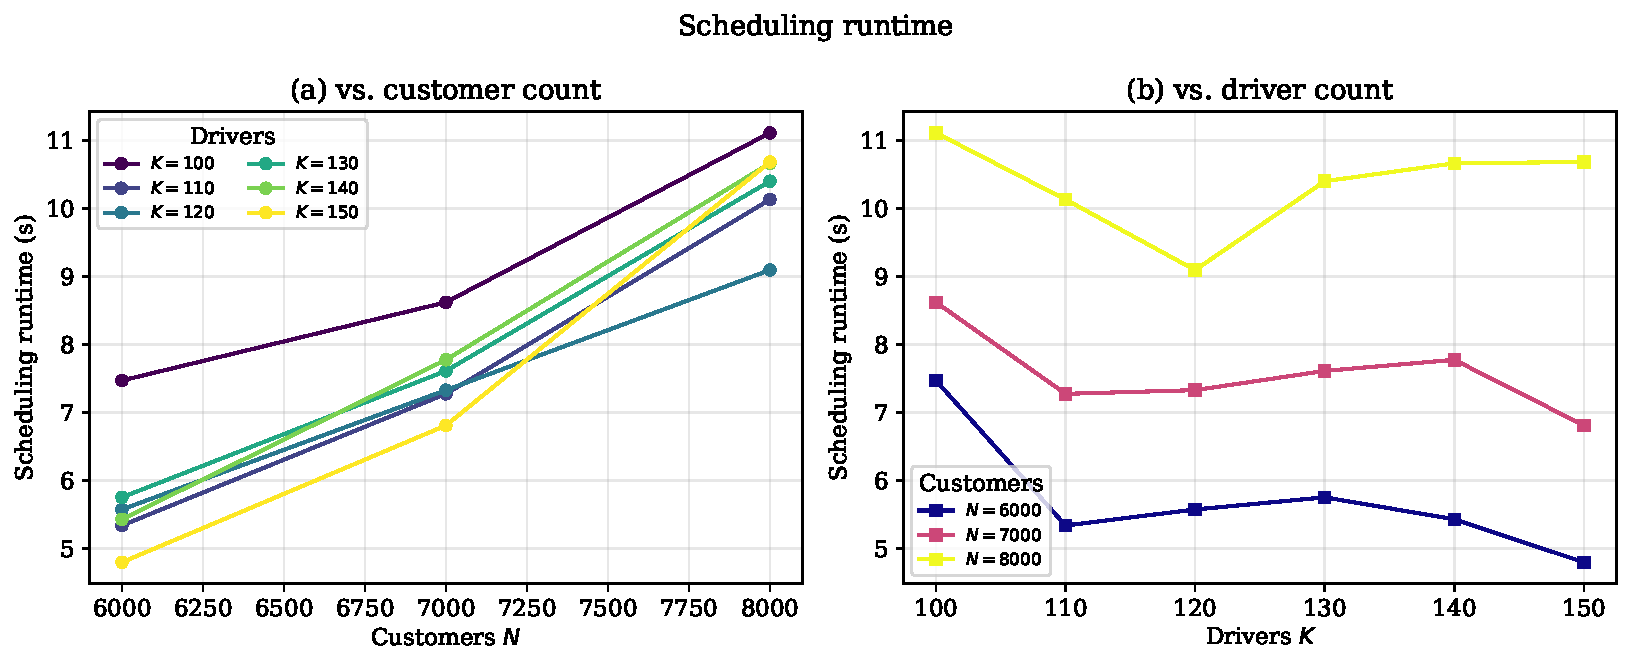
\includegraphics[width=\textwidth]{figures/results_scheduling_runtime.pdf}
  \caption{The runtime of the initial scheduling with respect to the number of customers and drivers}
  \label{fig:sched-runtime}
\end{figure}

The reference scenario with $N = 1000$ and $K = 200$ behaves differently. It is heavily over-provisioned, as only 166 of the 200 drivers serve any customers, and the average load is 4.1. Still, 326 customers remain unassigned. These customers likely cannot be served at all since a customer whose wanted pickup time falls late in the day fits inside the shift of only a small fraction of the drivers, and with on average 4.3 matched drivers per customer it is likely that none of them has a feasible start slot within the delay cap $E_{\max}$. Thus, the unassigned customers might not be a consequence of there being too few drivers. Instead this illustrates the possible effect of too strict preferences. With only one or two driver preferences, the risk of all preferred drivers not having a suitable ride slot becomes high.

\subsection{Conflict resolution results}

The last subproblem is the conflict resolution. From this subproblem, we record the objective value after the greedy assignment (initial) and after the iterated conflict resolution (final), the relative improvement between the two, the driver ordering that produced the best final objective, and the conflict resolution runtime $t_{\text{res}}$ in seconds. Table~\ref{tab:resolution} presents the results; Figure~\ref{fig:resolution-runtime} plots the runtime, Figure~\ref{fig:resolution-boxplot} compares the five driver orderings, and Figure~\ref{fig:objective-by-phase} shows the objective before and after the conflict resolution for every scenario.

\begin{table}[H]
\centering
\caption{Conflict resolution results}
\label{tab:resolution}
\small
\begin{tabular}{rrrrrlr}
\toprule
$N$ & $K$ & obj.\ initial & obj.\ final & improv.\ (\%) & strategy & $t_{\text{res}}$ \\
\midrule
1000 & 200 & 147704 & 163541 & -10.7 & load $\downarrow$ & 2.6 \\
6000 & 100 & 1464530 & 1288770 & +12.0 & load $\downarrow$ & 104.8 \\
6000 & 110 & 1454909 & 1280675 & +12.0 & index & 69.5 \\
6000 & 120 & 1408722 & 1209450 & +14.1 & load $\uparrow$ & 80.0 \\
6000 & 130 & 1383364 & 1171029 & +15.3 & index & 77.3 \\
6000 & 140 & 1365300 & 1146005 & +16.1 & confl. $\downarrow$ & 70.7 \\
6000 & 150 & 1329482 & 1102726 & +17.1 & confl. $\uparrow$ & 65.1 \\
7000 & 100 & 1757767 & 1575499 & +10.4 & index & 148.2 \\
7000 & 110 & 1742669 & 1547311 & +11.2 & confl. $\uparrow$ & 124.9 \\
7000 & 120 & 1681674 & 1481577 & +11.9 & confl. $\uparrow$ & 121.2 \\
7000 & 130 & 1647710 & 1422329 & +13.7 & confl. $\uparrow$ & 118.3 \\
7000 & 140 & 1624434 & 1378640 & +15.1 & confl. $\downarrow$ & 108.1 \\
7000 & 150 & 1596562 & 1335430 & +16.4 & confl. $\downarrow$ & 90.9 \\
8000 & 100 & 2047837 & 1863854 & +9.0 & load $\downarrow$ & 193.5 \\
8000 & 110 & 2009737 & 1803408 & +10.3 & load $\uparrow$ & 188.3 \\
8000 & 120 & 1980076 & 1765628 & +10.8 & confl. $\downarrow$ & 163.5 \\
8000 & 130 & 1950465 & 1720033 & +11.8 & confl. $\uparrow$ & 179.4 \\
8000 & 140 & 1926380 & 1688592 & +12.3 & load $\downarrow$ & 164.1 \\
8000 & 150 & 1883256 & 1612397 & +14.4 & confl. $\downarrow$ & 147.1 \\
\bottomrule
\end{tabular}
\end{table}

For all but the reference scenario, the iterated conflict resolution improves the objective by 9--17\,\%. The improvement grows with the number of drivers at every customer count, for example from 12.0\,\% at $K = 100$ to 17.1\,\% at $K = 150$ for $N = 6000$. This is expected as the conflict resolution improves the objective mainly by assigning previously unserved customers to drivers with spare capacity, each of which saves the penalty $P$, and a larger driver fleet has more spare capacity after the greedy pass. At a fixed number of drivers, the relative improvement decreases as the customer count grows, since the absolute gain stays similar while the objective itself grows with the number of unserved customers.

The resolution runtime grows superlinearly with the number of customers, from an average of 78 seconds at $N = 6000$ to 173 seconds at $N = 8000$, and decreases with the number of drivers (Figure~\ref{fig:resolution-runtime}), and it is roughly 15 times the first-pass runtime, as each of the five driver orderings reruns per-driver ILPs over several rounds. The runtime stays below 200 seconds in all scenarios.

\begin{figure}[H]
  \centering
  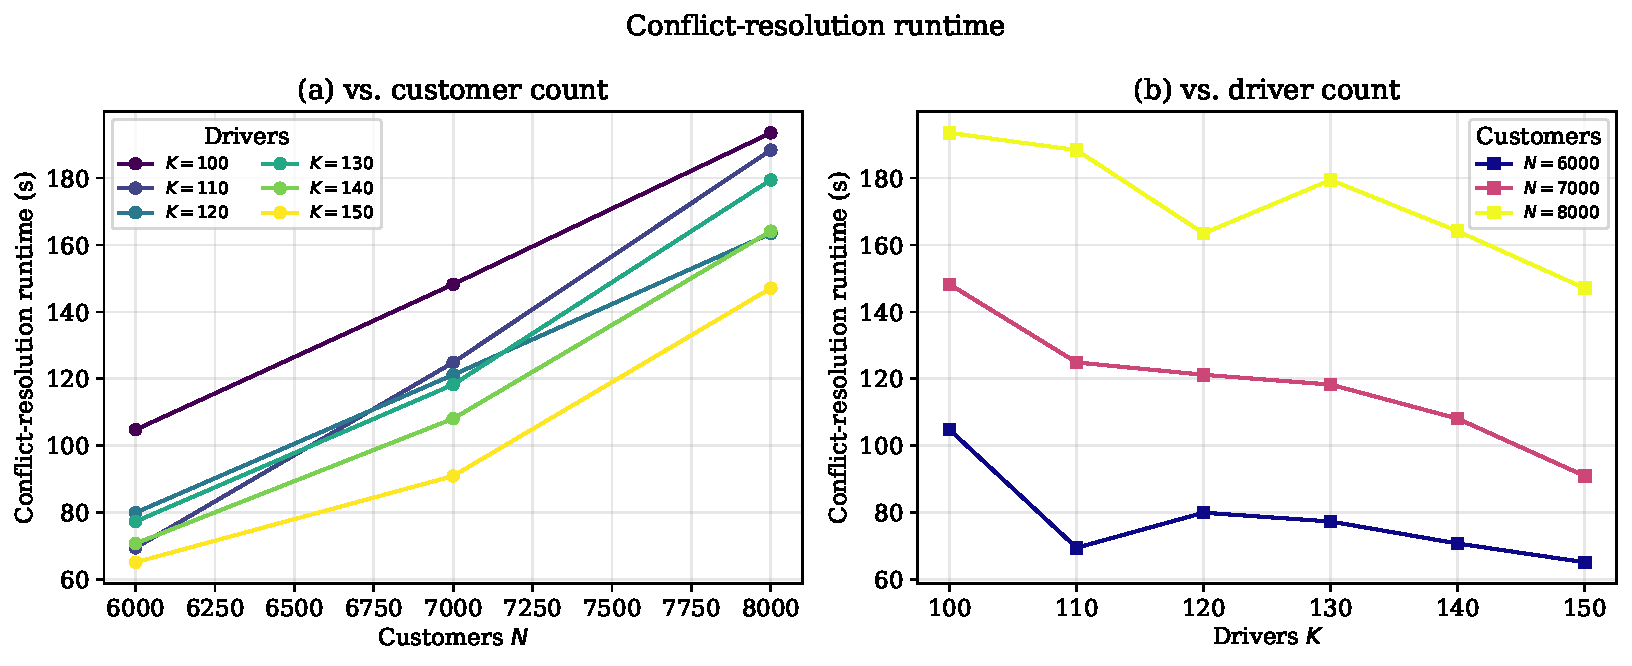
\includegraphics[width=\textwidth]{figures/results_resolution_runtime.pdf}
  \caption{The runtime of the conflict resolution with respect to the number of customers and drivers}
  \label{fig:resolution-runtime}
\end{figure}

Figure~\ref{fig:resolution-boxplot} shows that driver ordering matters little on average. The median excess over the per-scenario best ordering is below 0.11\,\% for every strategy, and no single ordering outperforms consistently, as shown in the chosen-strategy column of Table~\ref{tab:resolution}. The ascending-conflicts ordering has the lowest median excess, while the plain index ordering has the largest spread.

\begin{figure}[H]
  \centering
  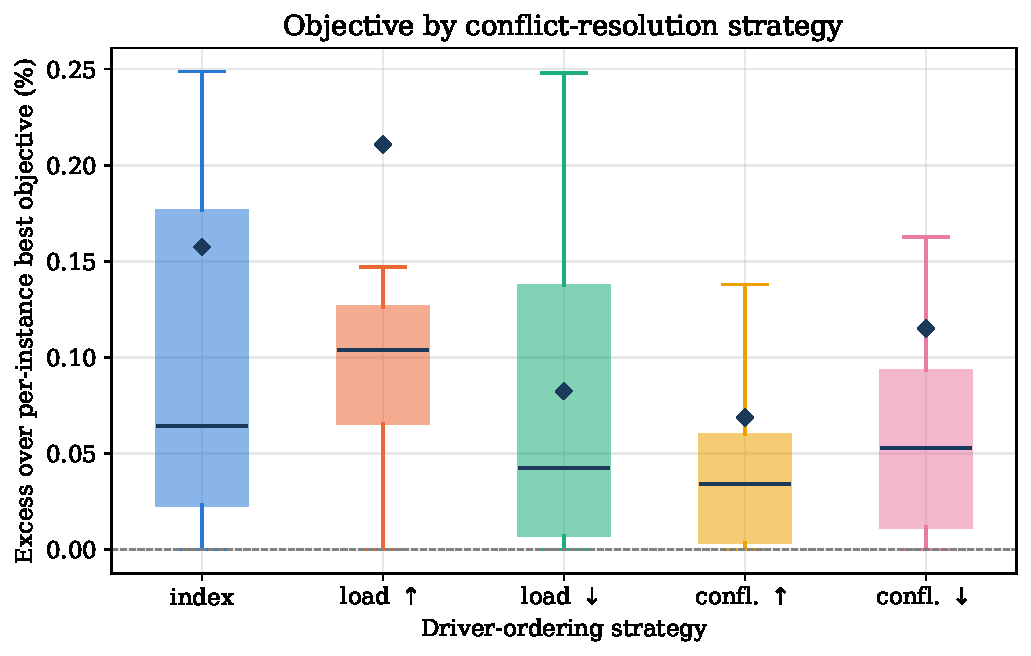
\includegraphics[width=\textwidth]{figures/results_resolution_boxplot.pdf}
  \caption{Excess of each driver-ordering strategy's objective over the per-scenario best. Outliers are omitted for readability.}
  \label{fig:resolution-boxplot}
\end{figure}

In the reference scenario, the resolution worsens the objective by 10.7\,\%. Each resolution is optimal for the driver itself but not necessarily
for the whole driver set. A driver assigned in the conflict resolution may drop a previously assigned customer back into the unserved pool, and in the over-provisioned reference scenario such swaps outweigh the few customers left to absorb them. The final result is the best of the five orderings; the initial greedy assignment is not kept as a candidate, so the pipeline does not fall back to it even when every ordering ends worse. Adding the greedy assignment as a sixth candidate would remove this failure mode.

\begin{figure}[H]
  \centering
  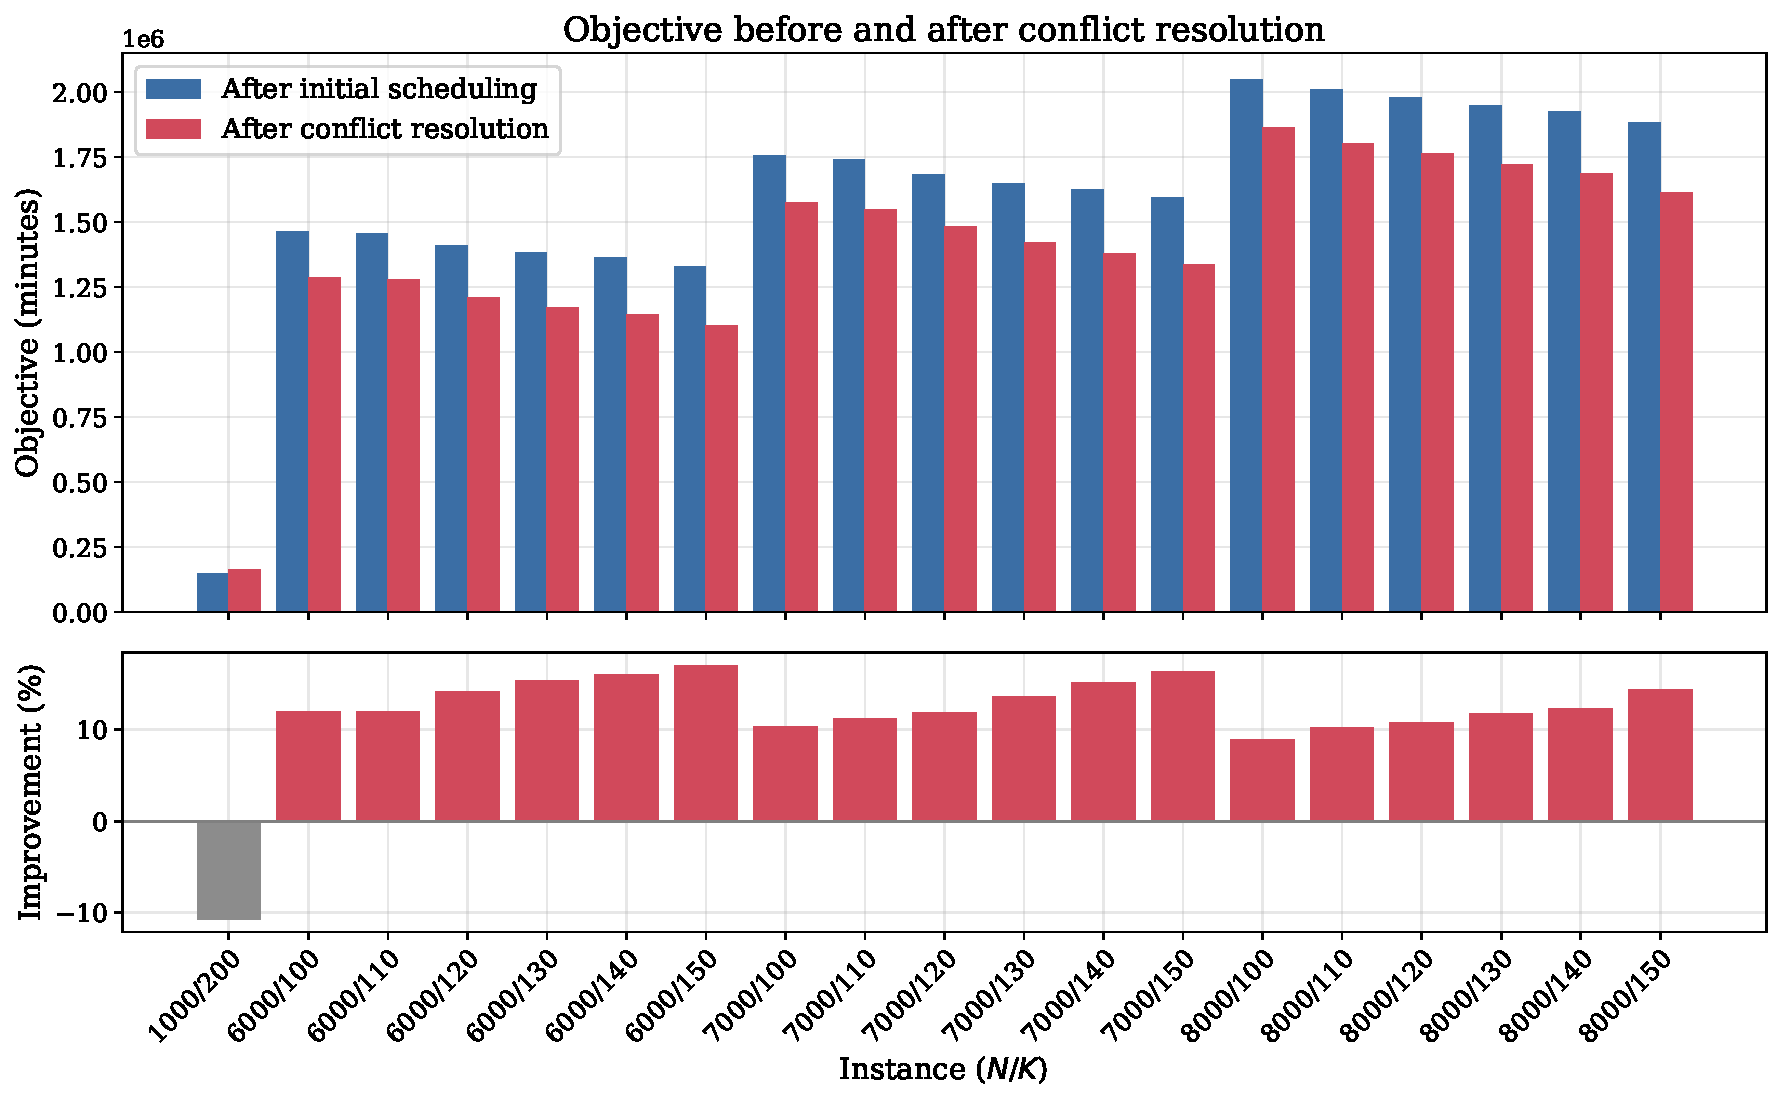
\includegraphics[width=\textwidth]{figures/results_objective_by_phase.pdf}
  \caption{Improvement of scheduling objective between the initial scheduling round and after resolving}
  \label{fig:objective-by-phase}
\end{figure}

\section{Conclusion}
\label{sec:conclusion}

In this thesis, we proposed a formulation of the multi-driver ride-sharing problem as a combination of separate single-driver scheduling problems. We modelled it as three subproblems: matching, scheduling, and conflict resolution. We formulated a three-step pipeline that first matches customers to drivers based on customer preferences, then finds each driver's schedule independently, and finally performs greedy conflict resolution to provide each driver's final conflict-free schedule. 

We found that the runtime of all three steps grows superlinearly with the number of customers. The matching and scheduling runtimes show no clear trend as the number of drivers increases, while conflict resolution becomes faster as the number of drivers increases. The scheduling step took the least time by far, at most a bit over 10 seconds, while conflict resolution took a little over 190 seconds for the scenario with 8000 customers and 100 drivers. The matching step took around 120 seconds for the largest scenarios. All in all, the largest scenarios took a bit over five minutes to solve.

Although it took a long time to solve, conflict resolution improved the objective value from the initial scheduling round by only 9--17\%. In the over-provisioned reference scenario with 1000 customers and 200 drivers, the conflict resolution step even worsened the result by almost 11\%. The solution was always optimal for the driver in question, given the current assignable set of customers, but not necessarily optimal for the entire driver fleet. Because the conflict resolution is greedy, the resulting schedules may not be optimal, and this effect can be amplified in customer-dense scenarios like the reference scenario. Also, because approximately 2/3 of customers were unserved in all but the reference scenario, all used scenarios are rather customer-dense. The order in which the driver resolves conflicts had almost no effect on the result, as the median excess over the per-scenario best ordering is below 0.11\% for all strategies. While the ascending conflicts ordering had both the smallest spread and median excess, no single ordering outperformed consistently.

As previously said, we investigated only one formulation of the ride-sharing problem. In our mathematical model, we considered only the time and coverage dimensions and modelled, for example, the distance dimension with a simple mandatory break between all rides. In reality, we would need to account for the time spent travelling between drop-off and pickup locations. Naturally, many more aspects could be investigated: traffic, travel cost, and the road network, to name a few. In the matching step, we considered only customer preferences. We could extend the preferences to include drivers' preferences, since some drivers may not want to serve certain customer types. The conflict resolution algorithm could also be improved to ensure a more globally optimal result. We could also improve the conflict-resolution metric, as our model used only pickup delay. In addition, we could improve the matching algorithm. We used Ford–Fulkerson with an Edmonds–Karp implementation, but improved algorithms already exist for solving maximum flow in a graph. \comments{A smoother ending}



%% LÄHDELUETTELO
%%  BibTeX-tiedoston kokoaminen onnistuu näppärästi esim. 
%%  Firefoxin/Chromen Zotero-lisäosalla http://www.zotero.org/
%%  joka osaa poimia viitteet suoraan Google Scholarista.

%% Ladataan library.bib
\bibliography{library}

%% Liitteet
%% Poista a.o. \clearpage-, \thesisappendix- ja input -makrot, jos liiteitä ei ole.
%% \clearpage
%% \thesisappendix

%% \input{sections/A-attachments}

\end{document}
